\chapter[Resultados Obtenidos]{Resultados obtenidos para los proplyds ``clásicos''}
\label{chap:proplyds}
\thispagestyle{empty}
Probamos nuestro modelo descrito en los capítulos anteriores en una muestra de proplyds pertenecientes a la Nebulosa de Orión (ONC) que presentan un choque de proa. En la figura \ref{fig:proplyds-map} se muestran los proplyds que pertenecen a nuestra muestra.

En todos los casos no fue posible medir el radio característico $R_{90}$ debido a que el brillo de la cáscara decae con el ángulo polar $\theta$ y no es detectable para ángulos del orden de $60^\circ$. Sin embargo, a continuación mostraremos la metodología para obtener la inclinación más probable de cada choque, así como los parámetros del modelo de cada uno de éstos que nos indican su forma intrínseca. Los resultados mostrados en este capítulo forman parte de un artículo por publicar.

\begin{figure*}
  \centering
    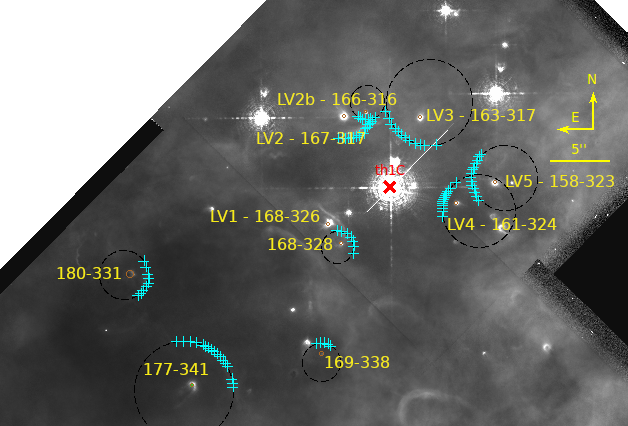
\includegraphics[width=\linewidth]{./Figures/Trapezium-annotate-rob-2018}
    \caption{Imagen de la parte central de la Nebulosa de Orión donde se ubican los proplyds de nuestra muestra. Las cruces color cyan corresponden a las mediciones de la forma aparente para cada choque de proa. Los círculos amarillos marcan la posición de cada proplyd y la ``x'' roja corresponde a la posición de la estrella ionizante \thC{}. Los círculos negros ilustran de manera esquemática el radio de curvatura de cada choque.}
    \label{fig:proplyds-map}
\end{figure*}

\section{Metodología para la medición de la forma aparente.}
\label{sec:methodology}
Se utilizaron imágenes en el filtro de [\Ion{O}{III}] de la cámara WPC2 del Telescopio Espacial Hubble (HST). Se utilizaron las herramientas del programa DS9 para análisis de imágenes astronómicas para trazar la posición de \thC{} y de cada uno de los proplyds de la muestra. La posición y la forma de los choques de proa fue trazada con una serie de marcas a lo largo del choque. Las coordenadas de las marcas fueron guardadas en un archivo y luego procesadas para tener las coordenadas del choque en el sistema de referencia del proplyd. El radio de curvatura aparente se obtiene haciendo un ajuste de mínimos cuadrados de la forma de un círculo de las mediciones obtenidas. $R_0$ se obtiene como la distancia a lo largo del eje $x$ entre el proplyd y el ajuste circular dentro del rango de las coordenadas de las mediciones. 

\subsection{Medición de incertidumbres}

Para saber qué tan confiables son las coordenadas de las mediciones, se realizó el procedimiento siguiente: Del total de marcas realizadas para trazar la posición del choque de cada proplyd, se crearon un total de 10 sub-muestras donde se removemos aleatoriamete aproximadamente una tercera parte de las marcas, pero dejando un mínimo de cuatro puntos, y se procedió a calcular los radios característicos para cada sub-muestra. La medición de la posición del choque sin restar marcas cuenta como la medición ``original'', y la diferencia entre la medición de los radios característicos para cada sub-muestra respecto a la muestra original será nuestra incertidumbre. En los casos de choques cuya forma se trazó con pocos puntos, las posibles sub-muestras que se pueden obtener son pocas respecto a otros choques donde se utilizaron más puntos, por tanto en estos casos habrá varias sub-muestras repetidas. En la figura \ref{fig:char-radii-obs} se muestran ejemplos de dichas sub-muestras para algunos proplyds.


\begin{figure*}
  \centering
  \setkeys{Gin}{width=0.5\linewidth}%, trim=10 30 55 62.5}
\begin{tabular}{cc}
 
Todos los puntos & Primera sub-muestra  \\ 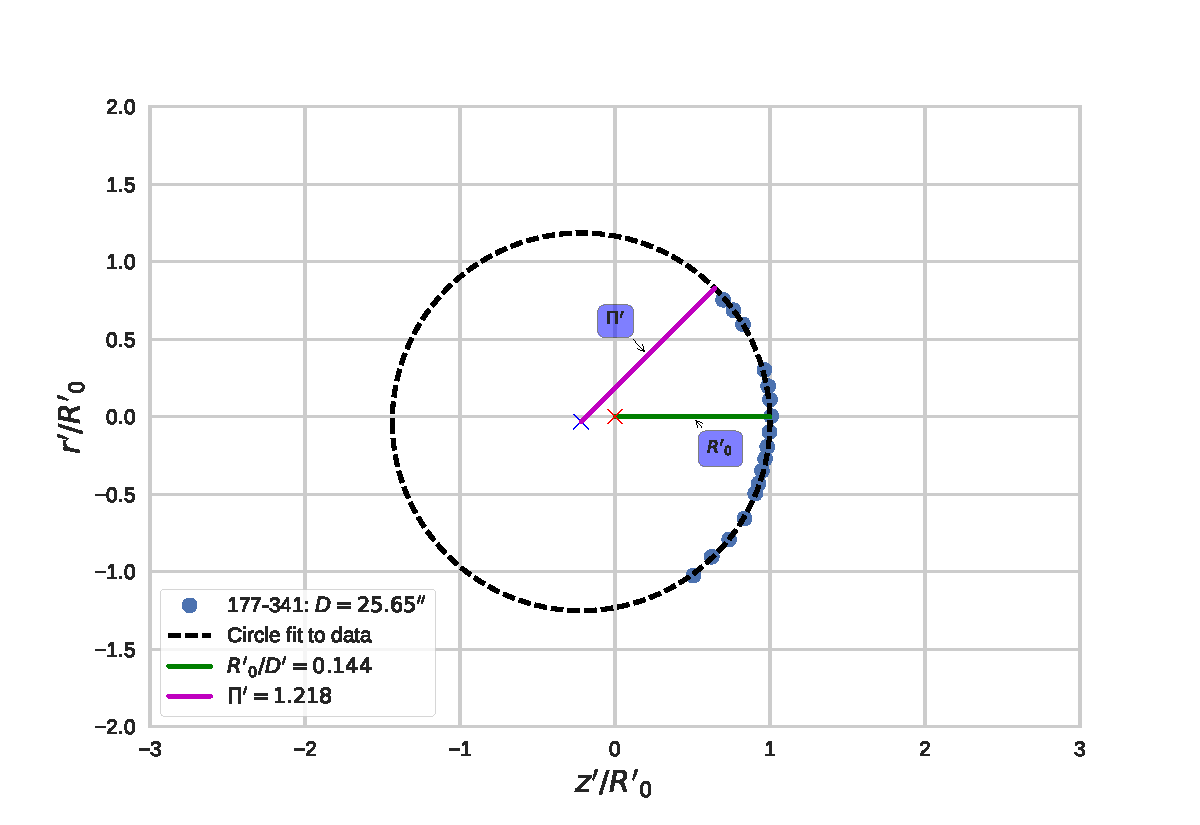
\includegraphics[clip]{./Programs/LV-bowshocks-xyfancy-positionswill-177-341} & 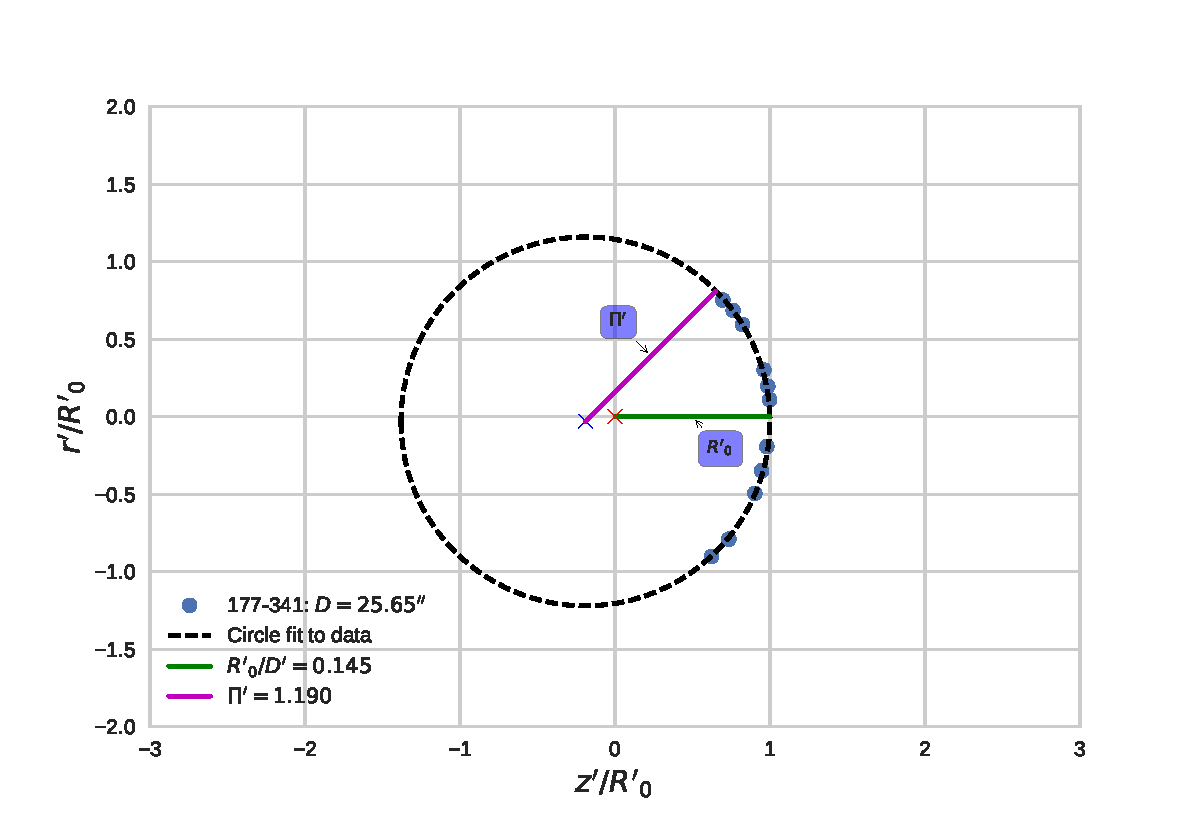
\includegraphics[clip]{./Programs/Multi-Fit/samp00/LV-bowshocks-xyfancy-positionssamp00-177-341} \\
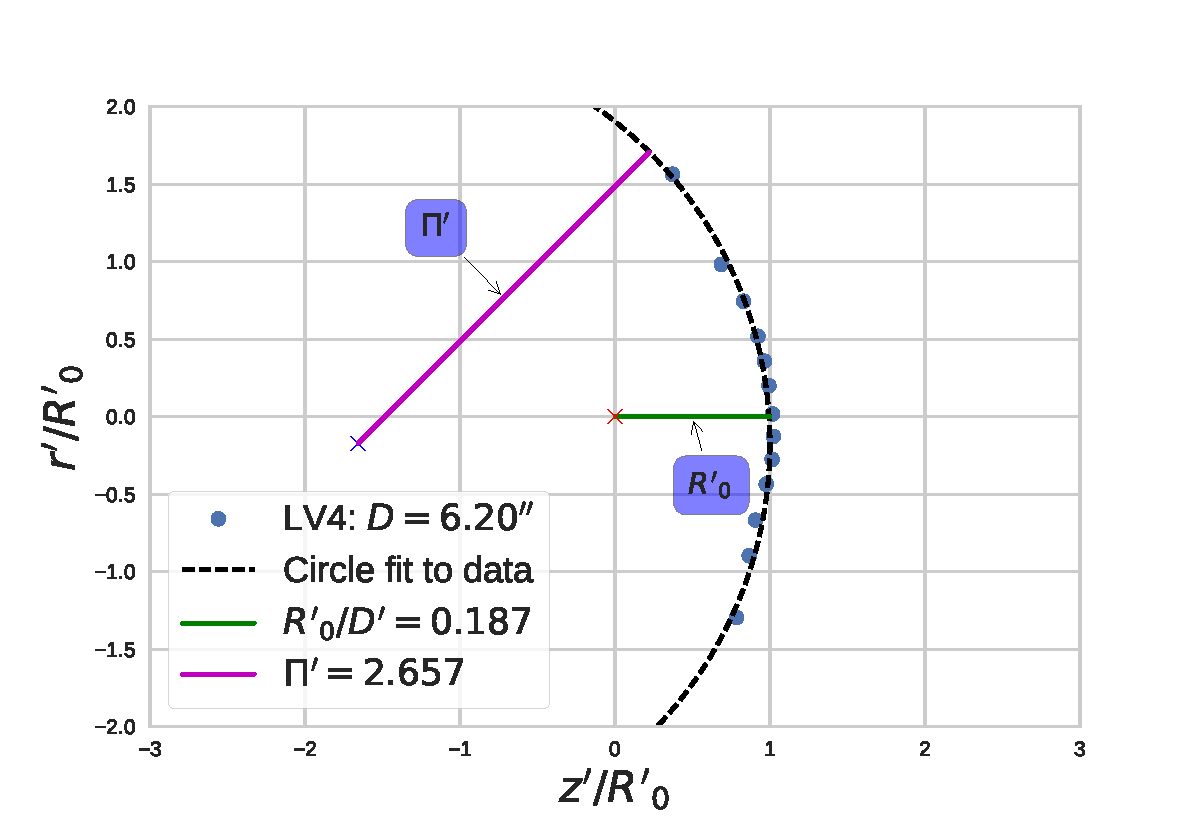
\includegraphics[clip]{./Programs/LV-bowshocks-xyfancy-positionswill-LV4} & 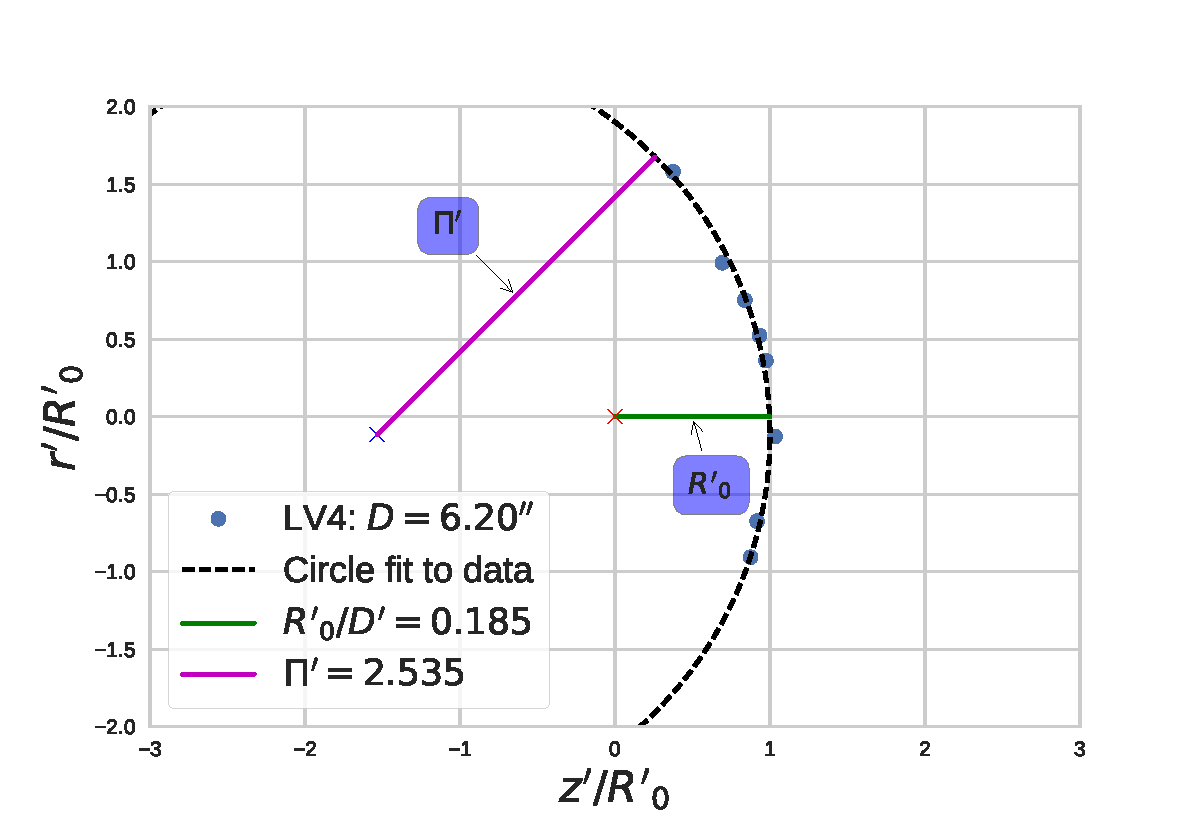
\includegraphics[clip]{./Programs/Multi-Fit/samp00/LV-bowshocks-xyfancy-positionssamp00-LV4} \\
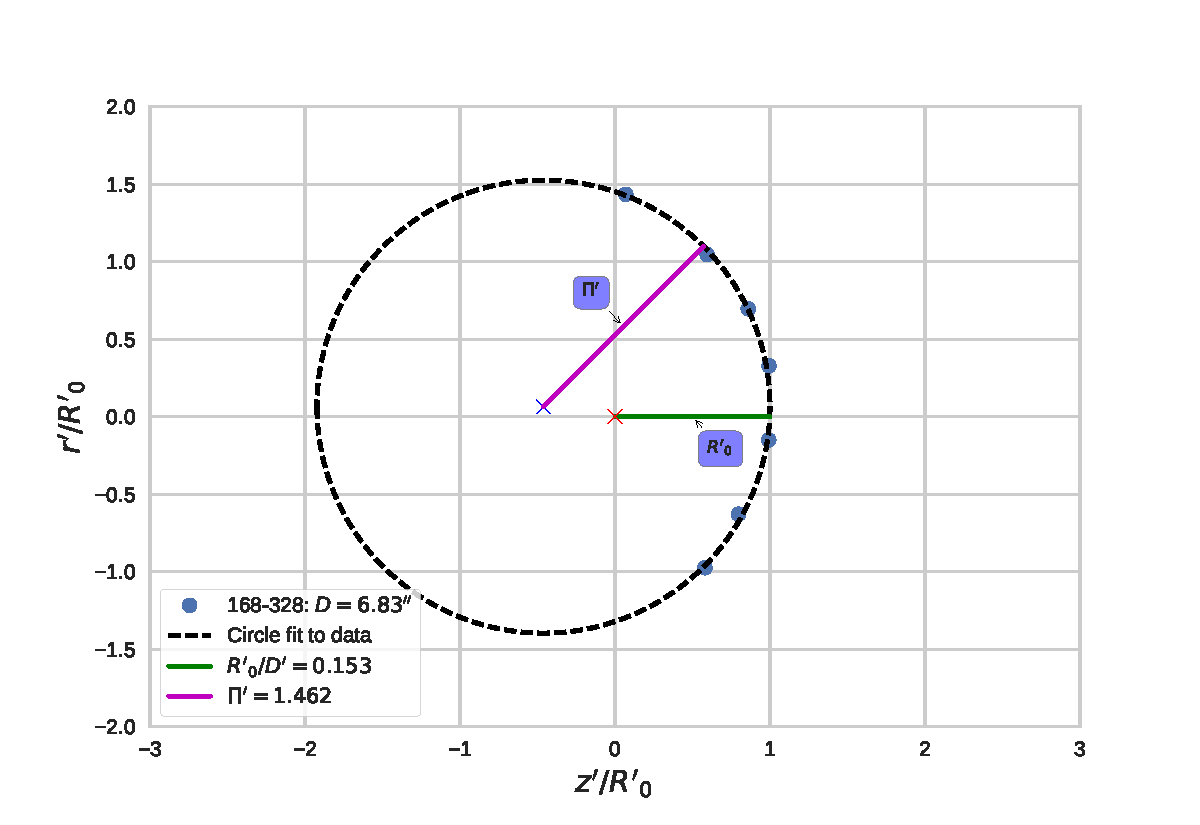
\includegraphics[clip]{./Programs/LV-bowshocks-xyfancy-positionswill-168-328} &  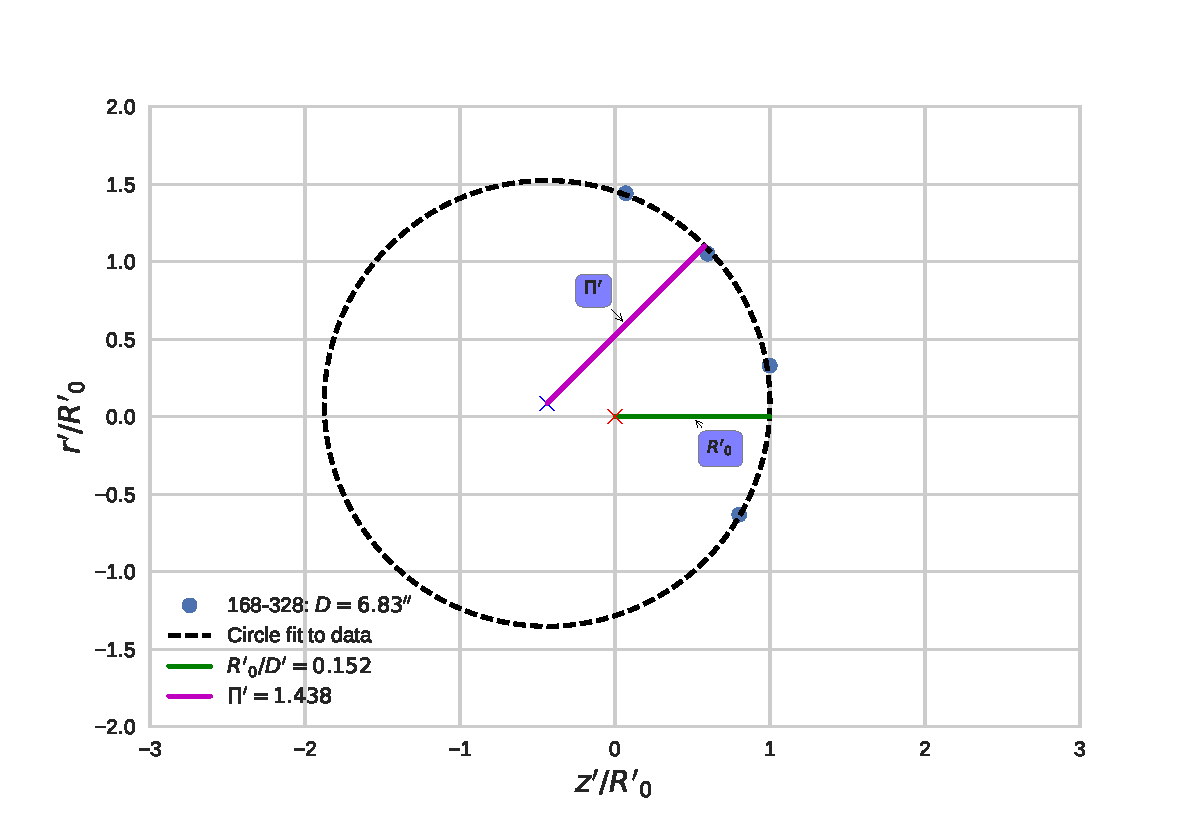
\includegraphics[clip]{./Programs/Multi-Fit/samp00/LV-bowshocks-xyfancy-positionssamp00-168-328} & 
\end{tabular}
\caption{Ejemplos de incertidumbres sistemáticas en los ajustes circulares a la forma de los choques para tres fuentes (desde la línea superior hasta la inferior): 177-341, LV4 y 168-328. La columna de la izquierda muestra el ajuste a todos los puntos identificados en el borde de la cáscara, donde el número y el espaciamiento de los puntos es una medida subjetiva de nuestra confianza al trazar el borde de cada cáscara. La columna de la derecha muestra el ajuste a una de las sub-muestras seleccionadas aleatoriamente que contienen 2/3 partes de los puntos de la muestra original para cada cáscara.}
\label{fig:char-radii-obs}
\end{figure*}

\begin{figure}
    \centering
  \ContinuedFloat
  \captionsetup{list=off,format=cont}
  \setkeys{Gin}{width=0.55\linewidth}
  \begin{tabular}{cc}
    Todos los puntos & Segunda sub-muestra  \\
    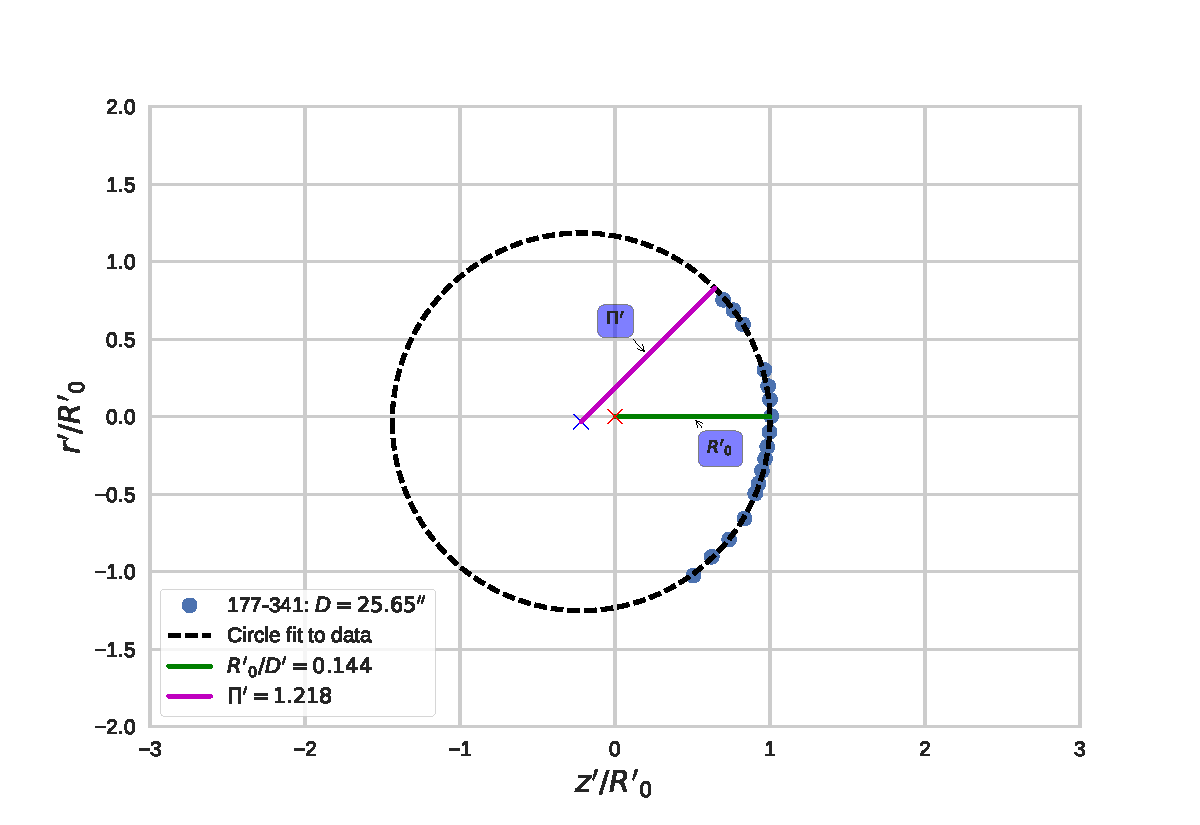
\includegraphics[clip]{./Programs/LV-bowshocks-xyfancy-positionswill-177-341} & 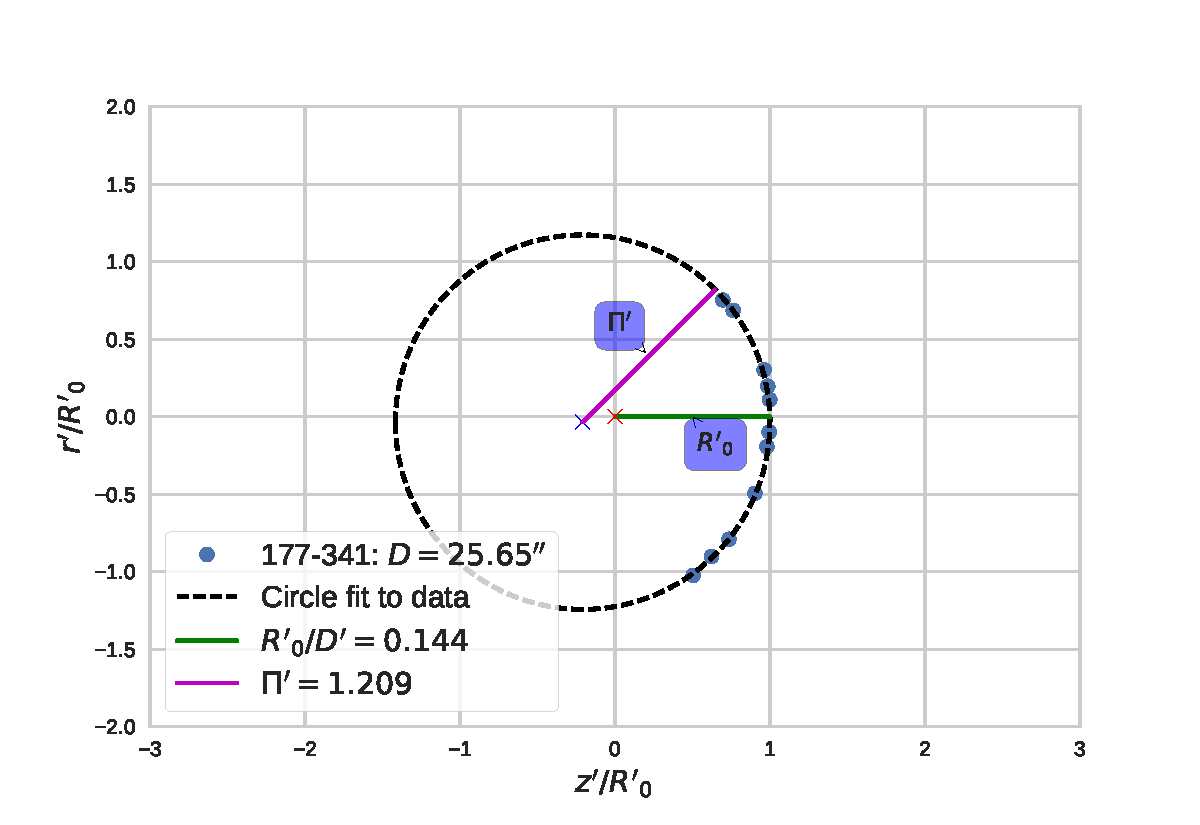
\includegraphics[clip]{./Programs/Multi-Fit/samp01/LV-bowshocks-xyfancy-positionssamp01-177-341} \\
    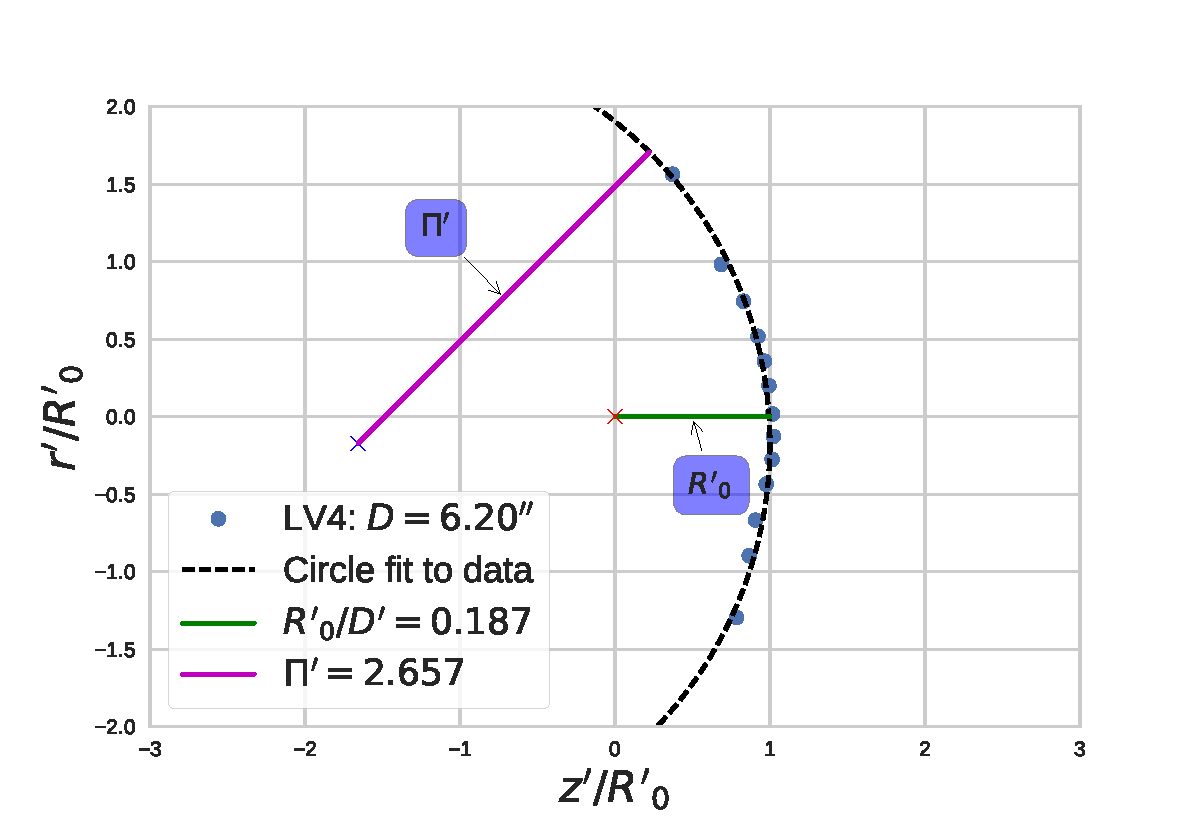
\includegraphics[clip]{./Programs/LV-bowshocks-xyfancy-positionswill-LV4} &                                                                            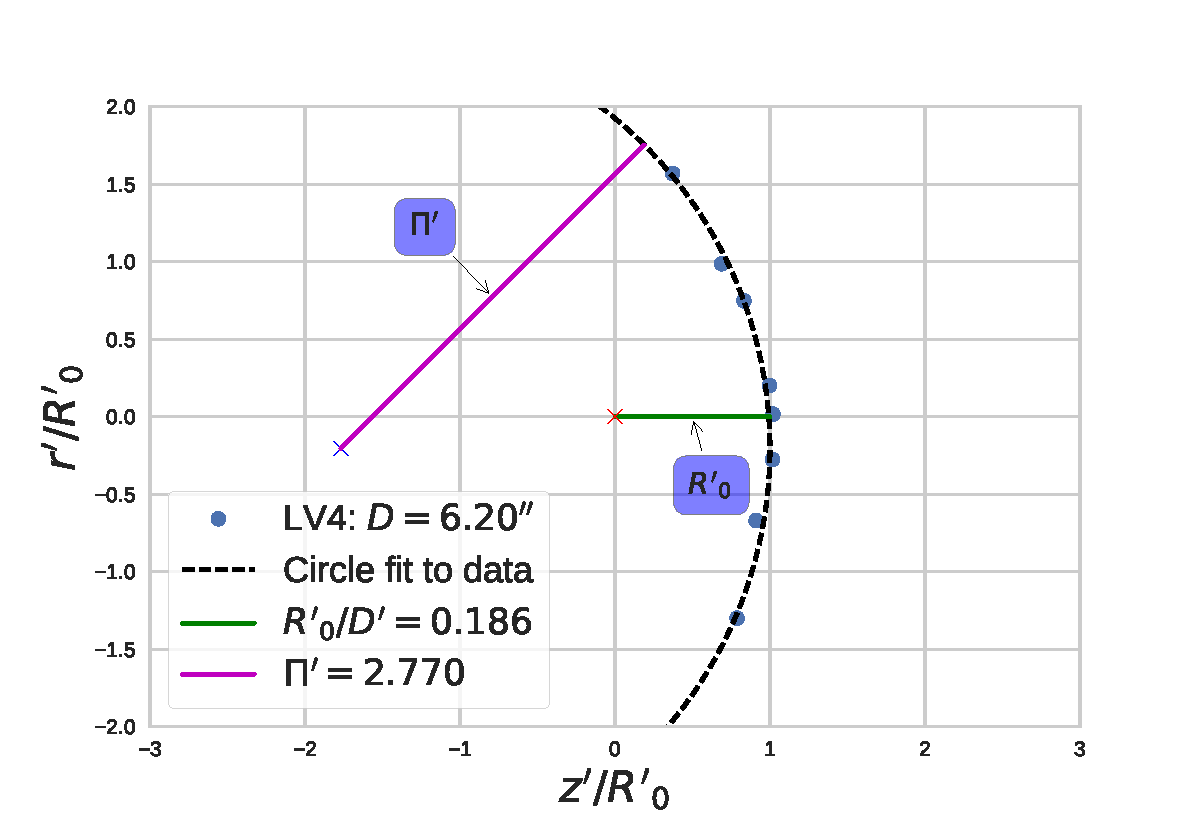
\includegraphics[clip]{./Programs/Multi-Fit/samp01/LV-bowshocks-xyfancy-positionssamp01-LV4} \\
    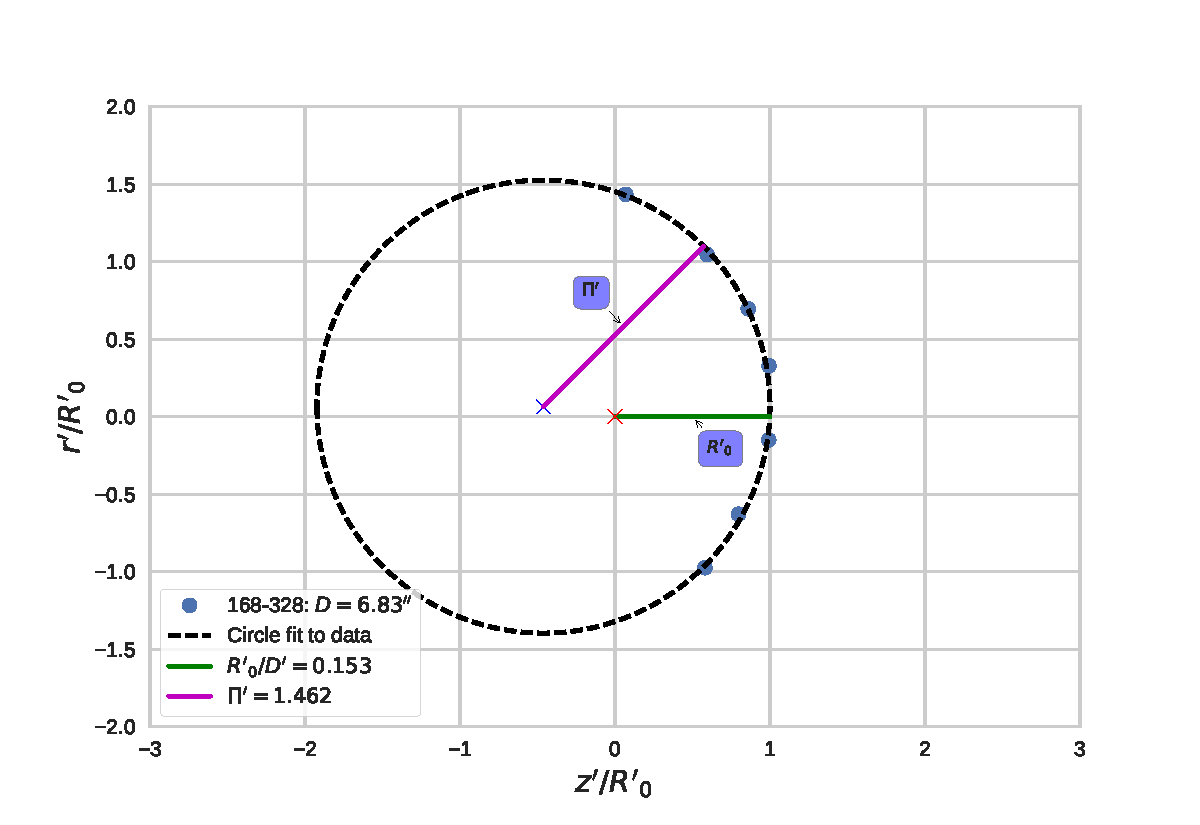
\includegraphics[clip]{./Programs/LV-bowshocks-xyfancy-positionswill-168-328} &
 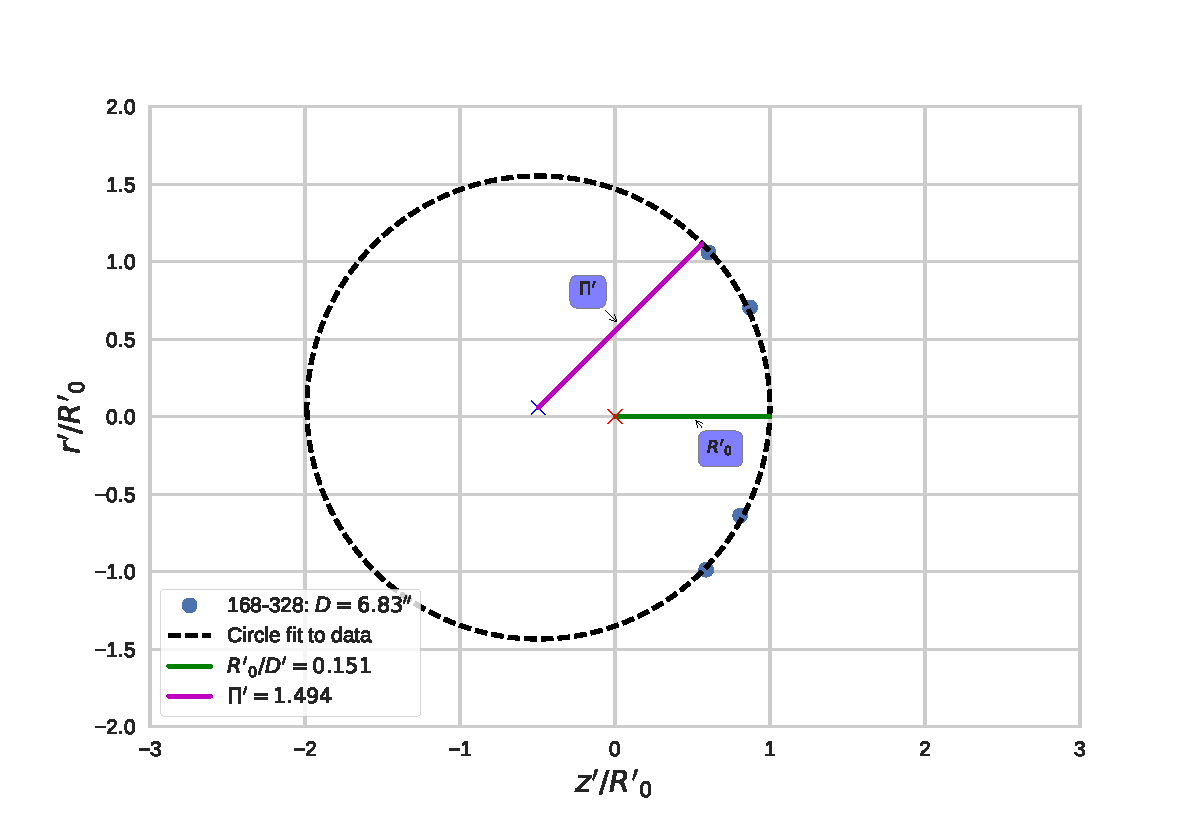
\includegraphics[clip]{./Programs/Multi-Fit/samp01/LV-bowshocks-xyfancy-positionssamp01-168-328}
    \end{tabular}
    \caption{En esta figura la columna de la derecha muestra el ajuste para una sub-muestra diferente a la columna anterior.}
\end{figure}


\section{Comparación con el Modelo de Capa Delgada}

Los radios característicos obtenidos para la muestra original y para las sub-muestras se muestran en la figura \ref{fig:obs-diagnostic}. En cada pánel se utiliza un valor fijo para el parámetro de anisotropía $k$. De estas figuras se pueden obtener la tasa de momentos $\beta$ y la inclinación $i$ para un grado de anisotropía dado por inspección visual al encontrar intersecciones entre las curvas teóricas y las barras radiales de las incertidumbres de cada proplyd (una por cada sub-muestra). Y a partir de éstos se puede inferir la distancia intrínseca a \thC{}, $D$, y el radio intrínseco en el ápex, $R_0$. En general algunas observaciones cualitativas que se encuentran son: Los proplyds con planitud mayor, LV4 y LV2b ajustan mejor a modelos donde el parámetro de anisotropía es bajo. LV2, quien tiene la planitud aparente más baja de toda la muestra, ajusta con modelos con alto índice de anisotropía $(k \gtrsim 3)$, con HST1 (177-341) ocurre algo similar, sin embargo, los modelos a los que ajusta este proplyd tienen una tasa de momentos baja e inclinaciones muy altas $(i \sim 80^{\circ})$. Esto es difícil de atribuirselo a errores en las mediciones por que es el proplyd que menos desviaciones tiene entre la medición original y las sub-muestras. El resto de los proplyds ajusta bien con un parámetro de anisotropía medio $(k\sim 1/2 - 3)$. Dependiendo de los parámetros $(\beta, k)$, la inclinación que se le puede atribuir a cada proplyd en la mayoría de los casos varía entre $15^\circ$ y $40^\circ$. 

\begin{figure}
  \centering
 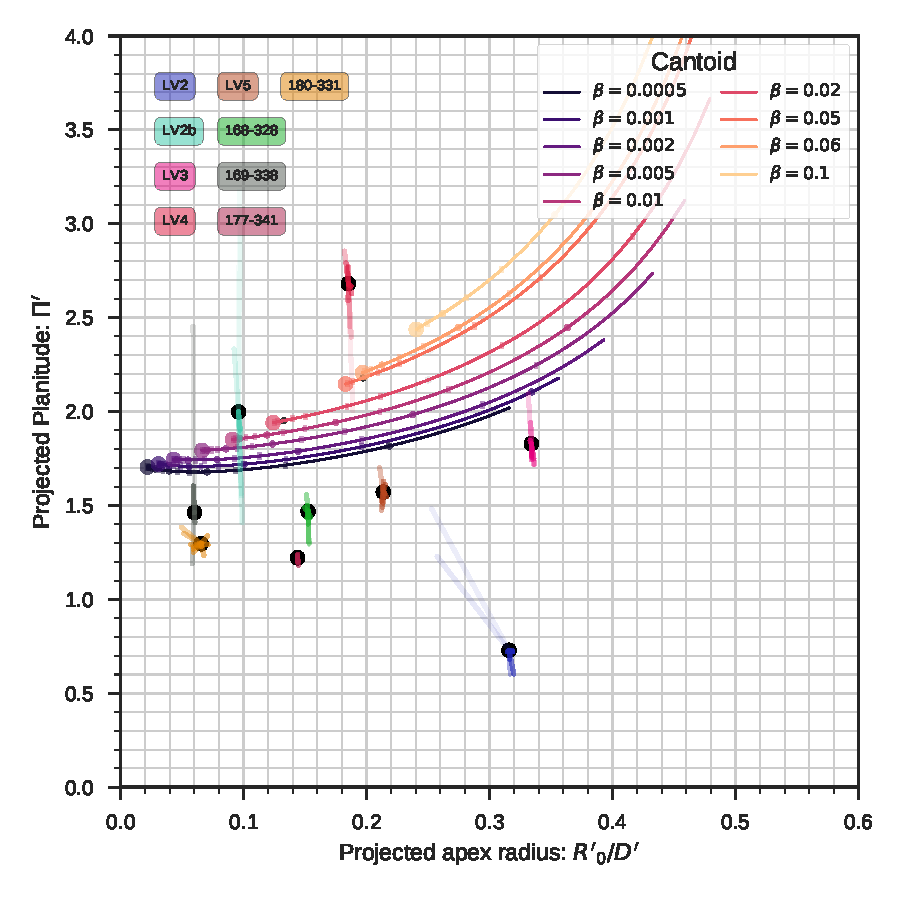
\includegraphics[width=0.9\linewidth]{./Figures/obs-diagnostic-Pi-R0-Cantoid}  
  \caption{Similar a la figura \ref{fig:Lambda-Pi-diagram} pero sustituyendo la alatud aparente por el radio aparente en el ápex $R'_0/D'$ para diferentes grados de anisotropía $k$, donde en cada pánel se asume que este parámetro es fijo. A lo largo de cada curva el valor del parámetro $\beta$ es fijo,  mientras que la inclinación se incrementa a lo largo de la curva, empezando a partir del círculo grande, donde $i=0^\circ$. Las marcas circulares pequeñas representan intervalos de $15^\circ$, mientras que las marcas más pequeñas representan intervalos de $5^\circ$. Los resultados observacionales de los choques de proa para nuestro set de proplyds se muestran con puntos negros, mientras que las mediciones de las sub muestras se muestran con líneas de colores radiales que parten desde la medición ``principal''. La opacidad de la medición de cada sub muestra es mayor cuanto menor sea la desviación respecto a la medición principal.}
  \label{fig:obs-diagnostic}
\end{figure}

\begin{figure}
  \centering
  \ContinuedFloat
  \captionsetup{list=off, format=cont}
  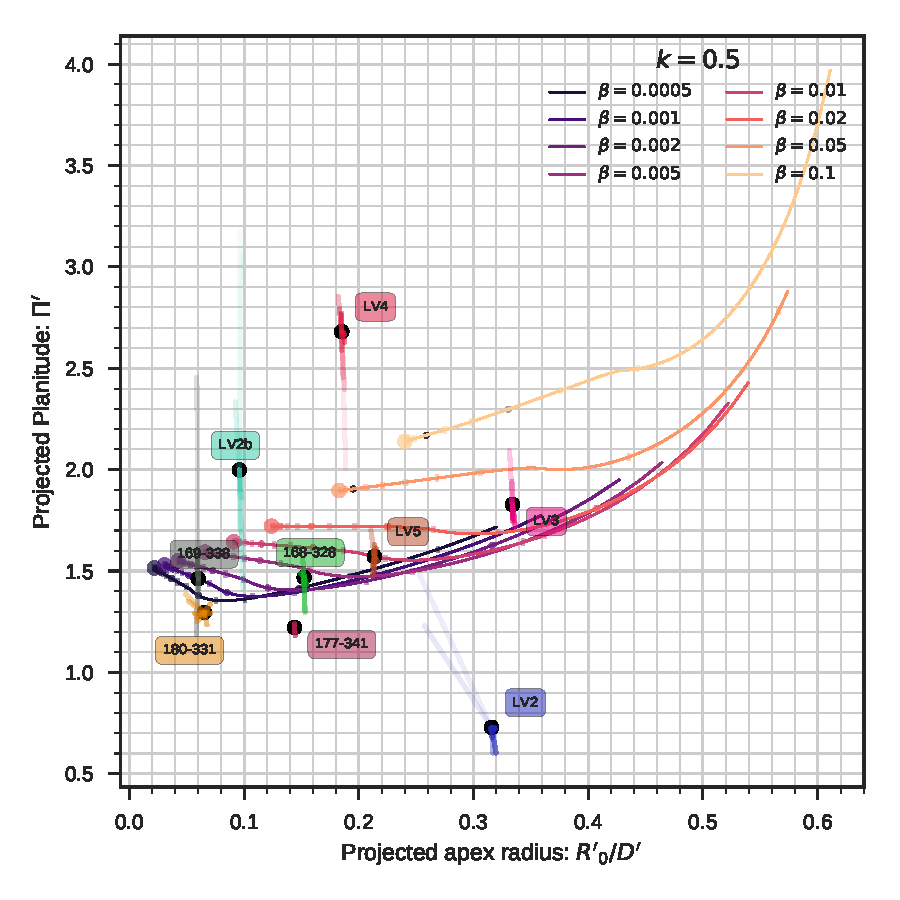
\includegraphics[width=0.9\linewidth]{./Figures/obs-diagnostic-Pi-R0-k05}
  \caption{}
  \label{fig:obs-diagnostic-2}
\end{figure}

\begin{figure}
  \centering
  \ContinuedFloat
  \captionsetup{list=off, format=cont}
  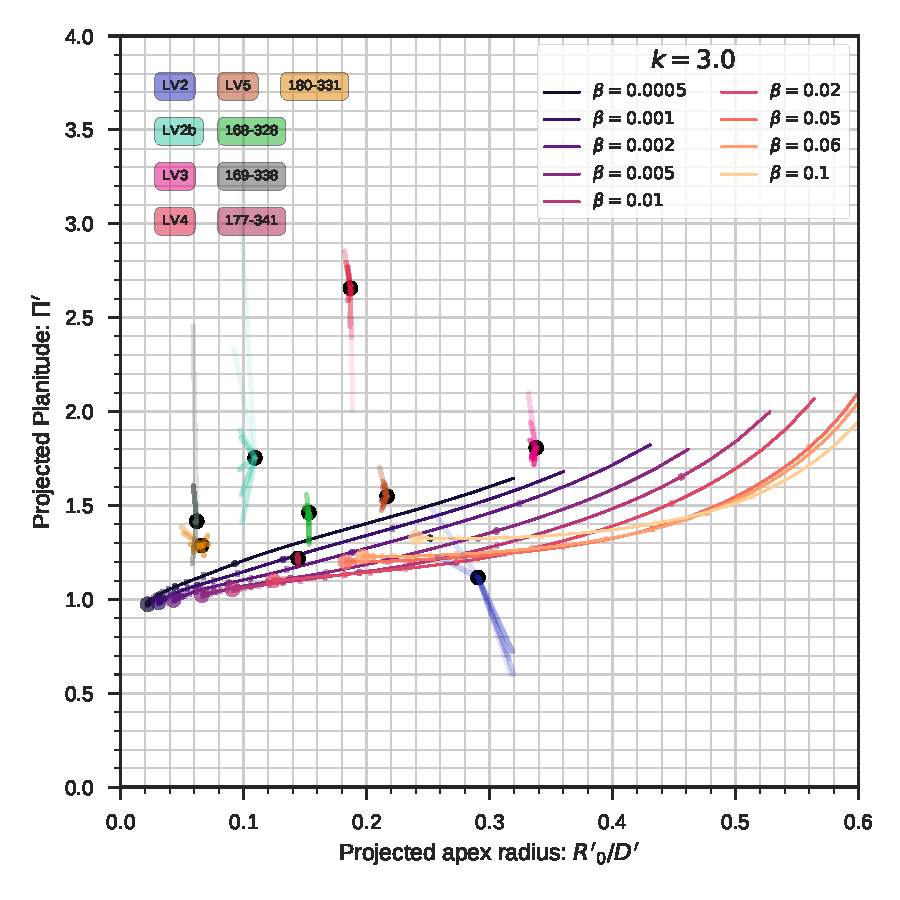
\includegraphics[width=0.9\linewidth]{./Figures/obs-diagnostic-Pi-R0-k30} 
  \caption{}
  \label{fig:obs-diagnostic-3}
\end{figure}

\begin{figure}
  \centering
  \ContinuedFloat
  \captionsetup{list=off, format=cont}
  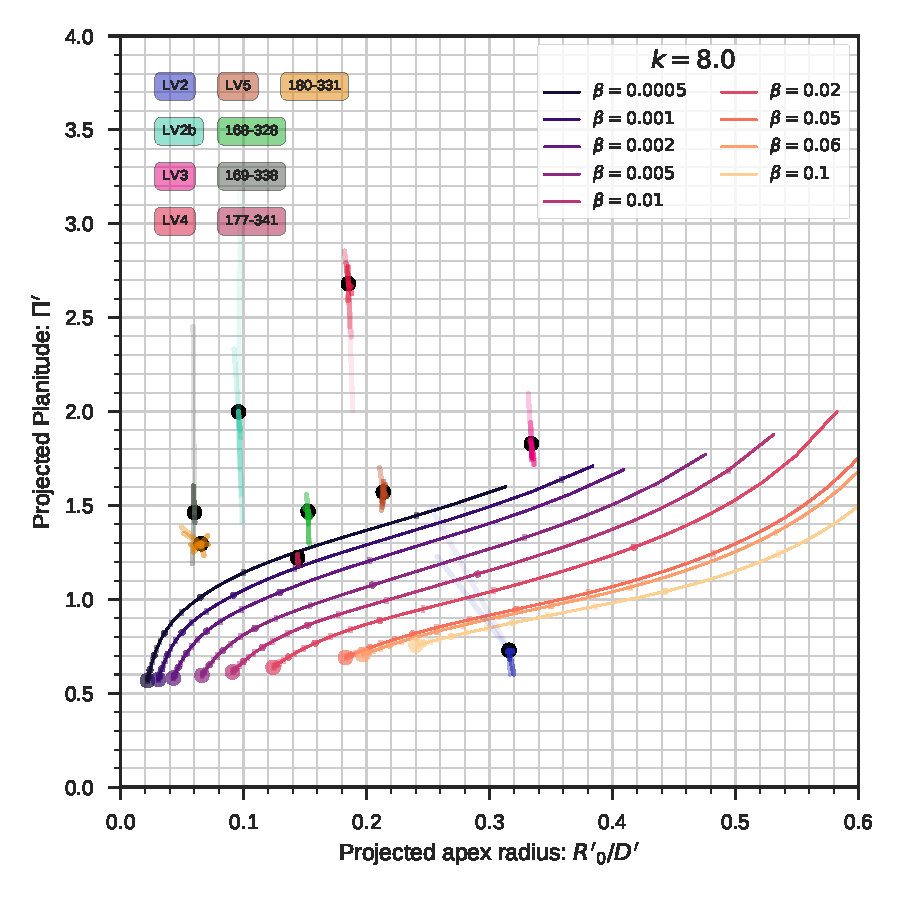
\includegraphics[width=0.9\linewidth]{./Figures/obs-diagnostic-Pi-R0-k80}
  \caption{}
  \label{fig:obs-diagnostic-4}
\end{figure}


%\begin{figure*}
%\begin{tabular}{cc}
%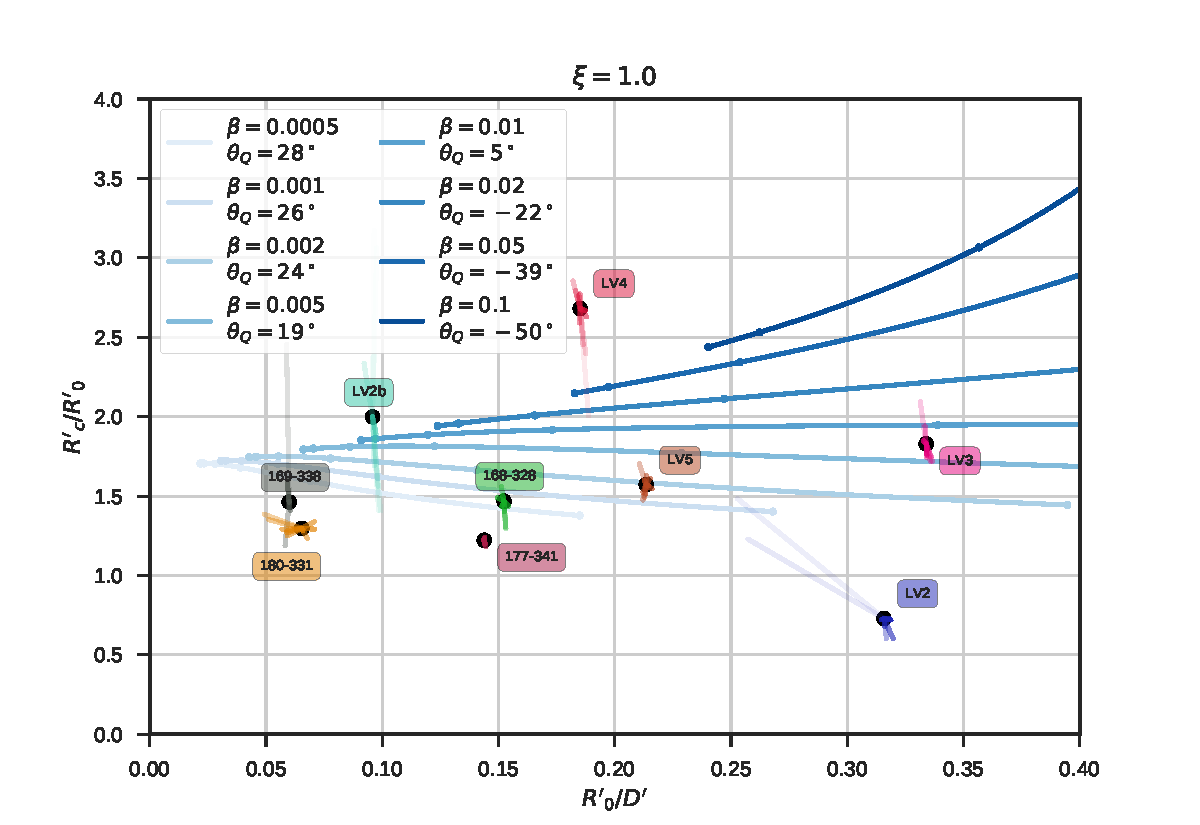
\includegraphics[width=0.48\linewidth]{./Figures/conic_xi-10} & 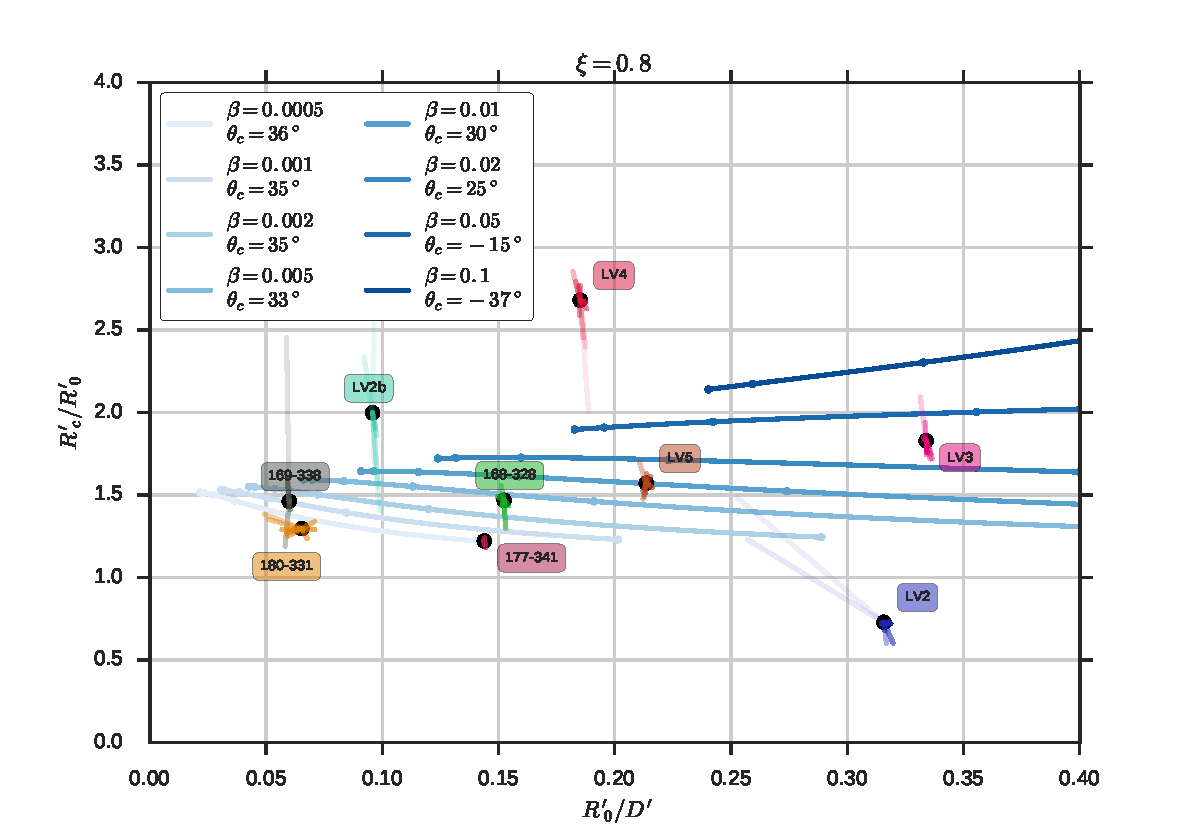
\includegraphics[width=0.48\linewidth]{./Figures/conic_xi-08} \\
%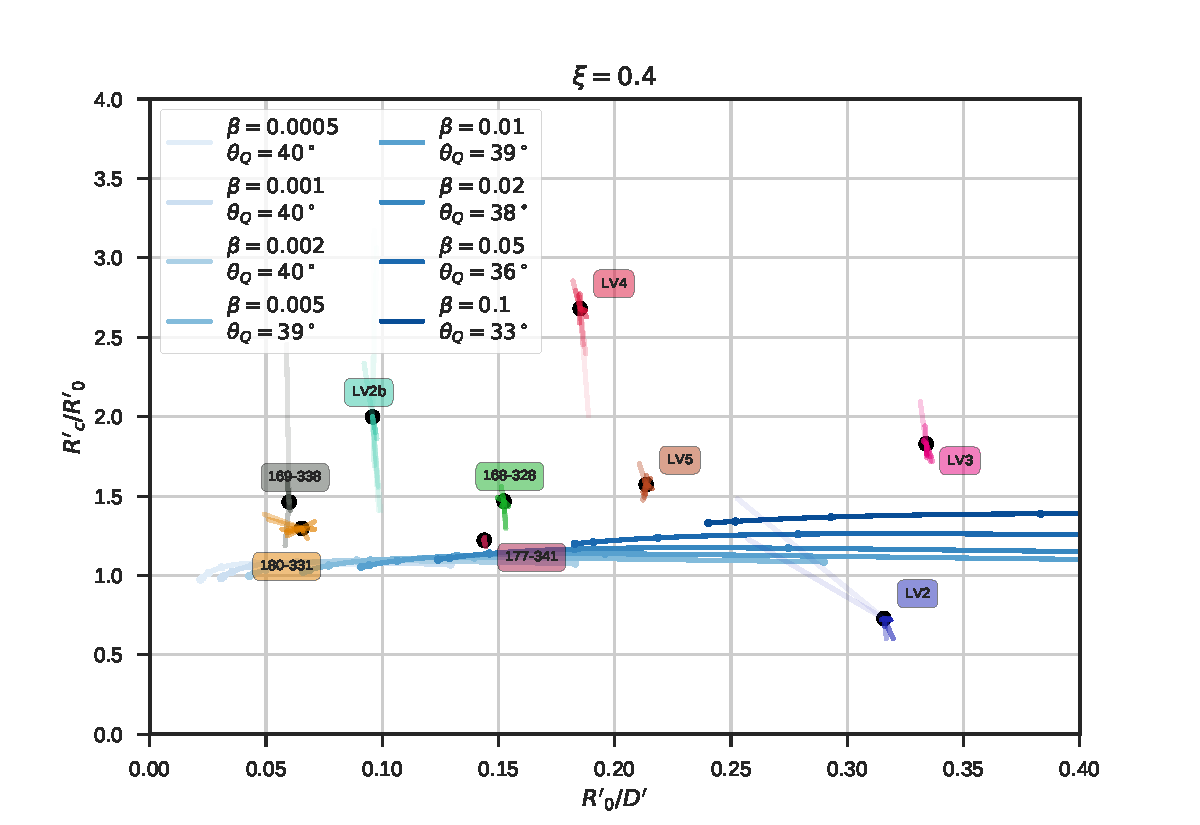
\includegraphics[width=0.48\linewidth]{./Figures/conic_xi-04} & 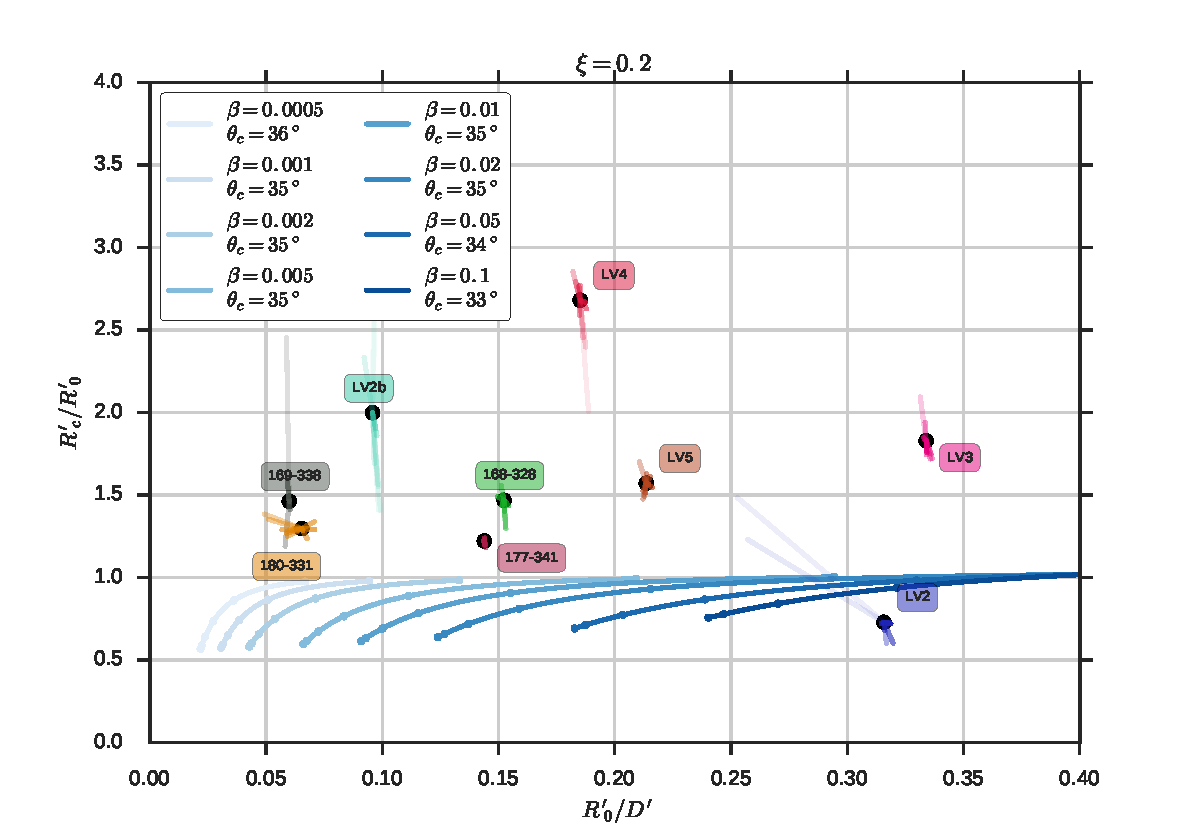
\includegraphics[width=0.48\linewidth]{./Figures/conic_xi-02} 
%\end{tabular}
%\caption{Mediciones de los radios característicos de los proplyds $R_c$ y $R_0$. Las curvas representan el ajuste de una cuádrica para un choque de proa con un cociente de momentos $\beta$ fijo, además se muestra su respectivo valor de $\theta_c$. Los puntos a lo largo de cada curva representan una separación en inclinación de $15^\circ$. Las mediciones para cada proplyd vienen acompañadas con el set de sub-muestras representadas como líneas radiales de colores. En cada gráfica se utiliza un valor diferente para el parámetro de anisotropía $\xi$, iniciando con un viento isotrópico $(\xi=1)$, hasta el viento  con mayor anisotropía $(\xi=0.2)$.}
%\label{fig:conic-xi}
%\end{figure*}

Con base a este análisis, se resume en la tabla \ref{tab:arc-fits} los ajustes a los parámetros de los proplyds: cociente de momentos $\beta$, inclinación, distancia a \thC{} intrínseca $D$ y radio del choque en el ápex $R_0/D$.
\begin{landscape}
  \begin{table*}
    \centering
  \caption{Ajuste a los parámetros de los arcos para los choques de proa de los proplyds}
  \label{tab:arc-fits} 
  \newcommand\C[1]{\multicolumn{1}{c}{#1}}
  \begin{adjustbox}{width=1.35\textwidth}
    \small
\begin{tabular}{llrllllrlll}\toprule
             &          & \multicolumn{3}{c}{\dotfill Observado \dotfill}              & \multicolumn{6}{c}{\dotfill Ajuste teórico \dotfill} \\ 
  \C{OW}     & \C{Nombre} & \(D'\) &\C{ \(R_0'/D'\) }&\C{ \(\Pi'_{\mathrm{shape}}\) }&\C{ \(\Pi'_{\mathrm{flux}}\) }&\C{ \(\beta\) }&\C{ \(k\) }&\C{ \(|i|\) }&\C{ \(D\) }&\C{ \(R_0/D\)}\\
  \C{(1)}& \C{ (2) }&\C{ (3)    }&\C{    (4)      }&\C{              (5)           }&\C{           (6)             }&\C{     (7)   }&\C{   (8)   }&\C{   (9) }&\C{  (10) }&\C{   (11)} \\
\midrule     
 168-328  &            &    6.8  &  $0.15 \pm 0.01$  &  $1.45^{+0.10}_ {-0.15}$   &  $1.55 \pm 0.05$     &  0.005  &  0.5  &  $52.5 \pm 2.50$   &  $0.022 \pm \SI{1.5e-3}{}$  &  $0.07$  \\
 169-338  &            &  16.4  &  $0.06 \pm 0.01$  &  $1.45^{+1.05}_{-0.25}$   &  $1.65 \pm 0.10$     &  0.002  &  0.0 -- 0.5  &  $36.3 \pm 1.25$   &  $0.040 \pm \SI{1.3e-3}{}$  &  $0.04$  \\
 177-341  & HST1   & 25.6  &  $0.15 \pm 0.01$  &  $1.25 \pm 0.05$   &  $1.15 \pm 0.05$     &  0.0005 -- 0.001  &  3.0 -- 8.0  &  $72.5 \pm 2.50$   &  $0.171 \pm \SI{2.6e-2}{}$  &  $0.04$  \\
 180-331  &             &  25.1  &  $0.07^{+0.01}_{-0.03}$  &  $1.30 \pm 0.10$   &  $1.30 \pm 0.10$     &  0.0005  &  0.5  &  $62.5 \pm 2.50$   &  $0.109 \pm \SI{2.2e-3}{}$  &  $0.02$  \\
 167-317  &  LV2     &    7.8  &  $0.29^{+0.03}_{-0.05}$  &  $1.15^{+0.35}_{-0.55}$   &  $1.03 \pm 0.18$      &  0.02 -- 0.1  &  3.0 -- 8.0  &  $42.5 \pm 2.04$  &  $0.021 \pm \SI{9.2e-4}{}$  &  $0.18 \pm 0.06$  \\
 166-316  & LV2b    &   7.2  &  $0.11^{+0.01}_{-0.03}$  &  $1.75^{+0.85}_{-0.35}$   &  $1.75 \pm 0.10$     &  0.02 -- 0.01  &  0.0 -- 0.5  &  $20.0 \pm 2.50$  &  $0.015 \pm \SI{4.4e-4}{}$  &  $0.11 \pm 0.02$  \\
  163-317  & LV3      &   6.9  &  $0.33 \pm 0.01$  &  $1.80^{+0.30}_{0.10}$   &  $2.05 \pm 0.05$     &  0.06  &  0.5  &  $40.0 \pm 2.50$   &  $0.018 \pm \SI{9.0e-4}{}$  &  $0.20$  \\
 161-324  & LV4      &   6.2  &  $0.19 \pm 0.01$  &  $2.65^{+0.25}_{-0.65}$   &  $2.10 \pm 0.05$     &  0.02 -- 0.05  &  0.0  &  $23.8 \pm 13.75$  &  $0.014 \pm \SI{1.7e-3}{}$  &  $0.15 \pm 0.03$  \\
 158-323  & LV5      &   9.6  &  $0.21 \pm 0.01$  &  $1.55 \pm 0.15$   &  $1.70 \pm 0.05$     &  0.02  &  0.5  &  $42.5 \pm 2.50$   &  $0.026 \pm \SI{9.4e-3}{}$  &  $0.02$  \\
\bottomrule
\end{tabular}
\end{adjustbox}
\begin{minipage}{0.95\linewidth}
%  \centering
\footnotesize
  Notas --
%
  Col.~(1): ID de la fuente \citep{ODell:1994a}.
%
  Col.~(2): Nombre alternativo de la fuente.
% 
  Col.~(3): Distancia proyectada desde \thC{}, segundos de arco.
%
  Col.~(4): Radio exterior aparente a lo largo del eje, normalizado con la distancia proyectada, donde la incertidumbre es calculada a partir de los valores máximo y mínimo de las submuestras descritas en \S~\ref{sec:methodology}, pero utilizando como mínimo la mitad de la resolución de los ejes de la figura \ref{fig:obs-diagnostic}. Se determina con el ajuste circular decrito en \S~\ref{sec:methodology}.
% 
  Col.~(5): Planitud aparente, donde la incertidumbre es calculada del mismo modo que en Col.~(4). Se determina con el ajuste circular descrito en \S~\ref{sec:methodology}.
% 
  Col.~(6): Planitud aparente, pero aplicando el criterio adicional de que el brillo superficial del proplyd obtenido debe coincidir con la predicción teórica. La medición central corresponde al promedio de las mediciones de las submuestras que cumplen con dicho criterio, con una desviación de $\pm 1\sigma$. Si solo una submuestra cumple el criterio, el resultado de Col.~(5) se traspasa a esta columna. 
%
  Col.~(7): Cociente de momentos entre el viento del proplyd y la estrella O (ver capítulo \ref{chap:hipersonica}) de las submuestras utilizadas en Col.~(6). 
% 
  Col.~(8): Parámetro de anisotropía del viento del proplyd.
% 
  Col.~(9): Inclinación respecto al plano del cielo, en grados.
% 
  Col.~(10): Distancia real desde \thC{}, parsecs.
%
  Col.~(11): Radio real de la cáscara a lo largo del eje, normalizado con distancia.

\end{minipage}
\end{table*}
\end{landscape}

\section{Obtención de la Presión de Equilibrio}

Las mediciones de los radios característicos y las inclinaciones obtenidas para los proplyds en esta sección se puede predecir la distancia intrínseca del proplyd $D$ a \thC{}, así como la escala intrínseca del proplyd, dada por el radio en el ápex $R_0$ (columnas 10 y 11 de la tabla \ref{tab:arc-fits}). Con ayuda de estos parámetros y además conociendo el radio del frente de ionización y la densidad máxima del flujo fotoevaporado en el frente de ionización de cada proplyd podemos estimar el flujo $F_*$ que se requiere para que exista equilibrio de ionización y compararlo con el flujo ionizante que recibe el proplyd de \thC{} a la distancia $D$. A su vez se puede estimar la presión ram del flujo fotoevaporado antes del choque y compararlo con la presión ram del viento estelar de \thC{} antes del choque. 


%Utilizamos los perfiles de brillo obtenidos en \citet{HA:1998} para obtener la densidad máxima y el radio del Frente de Ionización de nuestra muestra de proplyds. Sin embargo, a partir de los datos mostrados en la tabla 2 de dicho artículo, encuentro que utilizan una distancia a \thC{} de \SI{460}{pc}, mientras que en este trabajo utilizo una distancia de $414 \pm 6.8 \mathrm{~pc}$ \citep{Menten:2007}. En la tabla \ref{tab:prop-IF-par} muestro la densidad máxima y el radio del Frente de Ionización de nuestra muestra de proplyds corregidos por distancia a \thC{}, además, \citet{Henney:2001} encuentra que la densidad máxima obtenida en \citet{HA:1998} está sobreestimada por un factor del orden del 33\%.


\begin{table}
  % \begin{adjustbox}{width=\linewidth}
  \centering
  \caption{Parámetros del Frente de Ionización de los proplyds.}
  \label{tab:Prop-IF-par}
  \begin{tabular}{cccc} \toprule
    OW      & Nombre & $r_{\mathrm{IF}, 14}$*     & $N_6$* \\
    \midrule
    168-328 &        & $2.7 \pm 0.3$  & $4.08 \pm 0.48$ \\
    169-338 &        & $2.7 \pm 0.3$  & $1.43 \pm 1.09$ \\
    177-314 & HST1   & $19.6 \pm 1.9$ & $0.42 \pm 0.06$ \\ 
    180-331 &        & $11.7 \pm 1.3$ & $0.49 \pm 0.08$ \\
    167-317 & LV2    & $7.6 \pm 0.4$  & $2.65 \pm 0.23$ \\
    166-316 & LV2b   & $2.4 \pm 0.6$  & $4.21 \pm 1.21$ \\
    163-317 & LV3    & $4.8 \pm 0.7$  & $3.19 \pm 0.71$ \\
    161-324 & LV4    & $3.4 \pm 0.3$  & $4.21 \pm 0.63$ \\
    158-323 & LV5    & $6.1 \pm 0.7$  & $2.37 \pm 0.47$ \\
  \bottomrule
  \end{tabular}
  \begin{minipage}{0.9\linewidth}
%    \centering
    \footnotesize
    Notas --
%
  Col.~(1): ID de la fuente \citep{ODell:1994a}.
%
  Col.~(2): Nombre alternativo de la fuente.
%
  Col.~(3): Radio del IF del proplyd, en unidades de \SI{e14}{cm}
%
  Col.~(4): Densidad máxima del IF, en unidades de \SI{e6}{cm^{-3}}
%
  * En la Col.~(3) la corrección por distancia se da como sigue: $r_{\mathrm{IF}, 14} = r_{\mathrm{IF}, 14}^{\mathrm{GAH}}\frac{\SI{414}{pc}}{\SI{430}{pc}}$, mientras que en la Col.~(4) la corrección es $N_6 = N_6^{\mathrm{GAH}}\left(\frac{\SI{414}{pc}}{\SI{430}{pc}}\right)^{-1/2}$, donde $r_{\mathrm{IF}, 14}^{\mathrm{GAH}}$ y $N_6^{\mathrm{GAH}}$ son el radio del frente de ionización medido en unidades de \SI{e14}{cm} y su densidad medida en unidades de \SI{e6}{cm^{-3}} extraídos de \citet{Garcia-Arredondo:2001}.
  \end{minipage}
\end{table}

El flujo de fotones ionizantes necesario para que exista equilibrio de ionización en el flujo fotoevaporado proveniente del proplyd, se puede determinar con la siguiente ecuación \citep{Henney:2001}:

\begin{align}
  F_{\mathrm{ph}} = v_w(r_{\mathrm{IF}}) n_{\mathrm{IF}} + \alpha'_{\mathrm{rec}}n^2_{\mathrm{IF}} \omega r_{\mathrm{IF}}\label{eq:F-ph}
\end{align}

Donde $\alpha'_{\mathrm{rec}} = \SI{2.6e-13}{cm^3.s^{-1}}$ (ver apéndice \ref{app:HII}), $\omega \simeq 0.12$ es un factor que está relacionado con la ley de velocidades del flujo fotoevaporado del proplyd, y es proporcional al grosor del IF escalado con $r_{\mathrm{IF}}$, $n_{\mathrm{IF}}$ es la densidad máxima del frente de ionización, y por último, estamos considerando que los frentes de ionización son de tipo D crítico, de donde se obtiene que $v_w(r_{\mathrm{IF}}) = c_{\mathrm{II}} = \SI{11}{km.s^{-1}}$, donde $a_{\mathrm{II}}$ es la velocidad del sonido del medio ionizado.

Por otro lado, el flujo de fotones ultravioleta provenientes de \thC{} a la distancia $D$ viene dado por:

\begin{align}
   F_* &= \frac{(1-f_d)\Nio_*}{4\pi D^2} \label{eq:F-star} 
\end{align}

Donde $f_d$ es un factor relacionado con la absorción del polvo.

La condición de equilibrio de ionización implica que $F_{ph} = F_*$. Sin embargo, no todas las mediciones de las submuestras predicen una distancia $D$ que lleven a alcanzar dicho equilibrio. En la columna (6) de la tabla \ref{tab:arc-fits} mostramos el promedio de la planitud aparente de las sub-muestras que se aproximan más al equilibrio de ionización, y para las mediciones consecuentes de dicha tabla (columnas (7) en adelante) también se utilizan estas sub-muestras.

Por otro lado, la presión ram en la cáscara viene dada por:

\begin{align}
  P_{in} = n_{ps}\bar{m}c_{\mathrm{II}}^2M^2 \label{eq:P-in}
\end{align}

donde $\bar{m} = \mu m_p$, donde $\mu = 1.3$ para un gas con una temperatura de $\sim \SI{e4}{K}$ y una velocidad del sonido de \SI{11}{km.s^{-1}}, $m_p = \SI{1.673e-24}{g}$ es la masa del hidrógeno, $M$ es el número de Mach del flujo fotoevaporado antes del choque y $n_{ps}$ es la densidad máxima del flujo fotoevaporado antes del choque, que se relaciona con $n_{\mathrm{IF}}$ como sigue:

\begin{align}
  n_{ps} = n_{\mathrm{IF}}\left(\frac{R_0}{r_{\mathrm{IF}}}\right)^{-2} M^{-1} \label{eq:density-scale}
\end{align}


Por último, la presión ram del viento de \thC{} en función de la distancia radial $r$ es:

\begin{align}
  P_*(r) = \frac{\dot{M}^{0}_{w1}v_{w1}}{4\pi r^2} \label{eq:P-star}
\end{align}

%Donde $\dot{M}^{0}_{w1} = \SI{3.5e-7}{M_\odot.yr^{-1}$ es la tasa de pérdida de masa de \thC{}, y $v_{w1} = \SI{1400}{km.s^{-1}}$ es la velocidad terminal del viento de \thC{}.
 Donde $\dot{M}^{0}_{w1}$ es la tasa de pérdida de masa de \thC{} y $v_{w1}$ es la velocidad terminal del viento. De manera análoga al flujo, el equilibrio de presiones ram que implica un choque estacionario se logra cuando $P_{in} = P_*$, y esto ocurre para cada proplyd cuando $r = D-R_0$. %En la figura \ref{fig:wind-fits} se hace una comparación entre $F_{ph}$, $P_{in}$, $F_*$ y $P_{*}$ vs $D$ en un diagrama log-log para las sub-muestras que cumplen con la condición $\left|\frac{F_{ph}}{F_*}\right| < 10$. %Para los proplyds más lejanos se observa que las mediciones de las submuestras disponibles predicen una presión RAM mayor a la que se requiere para que el choque sea estacionario. Esto puede significar que por su distancia a \thC{} la presión del viento estelar deja de ser dominante y otra fuente también contribuye a confinar el choque de proa de estos proplyds. Esta hipótesis se está trabajando en un artículo por publicar.


\begin{figure}
  \centering
  \begin{tabular}{cc}
    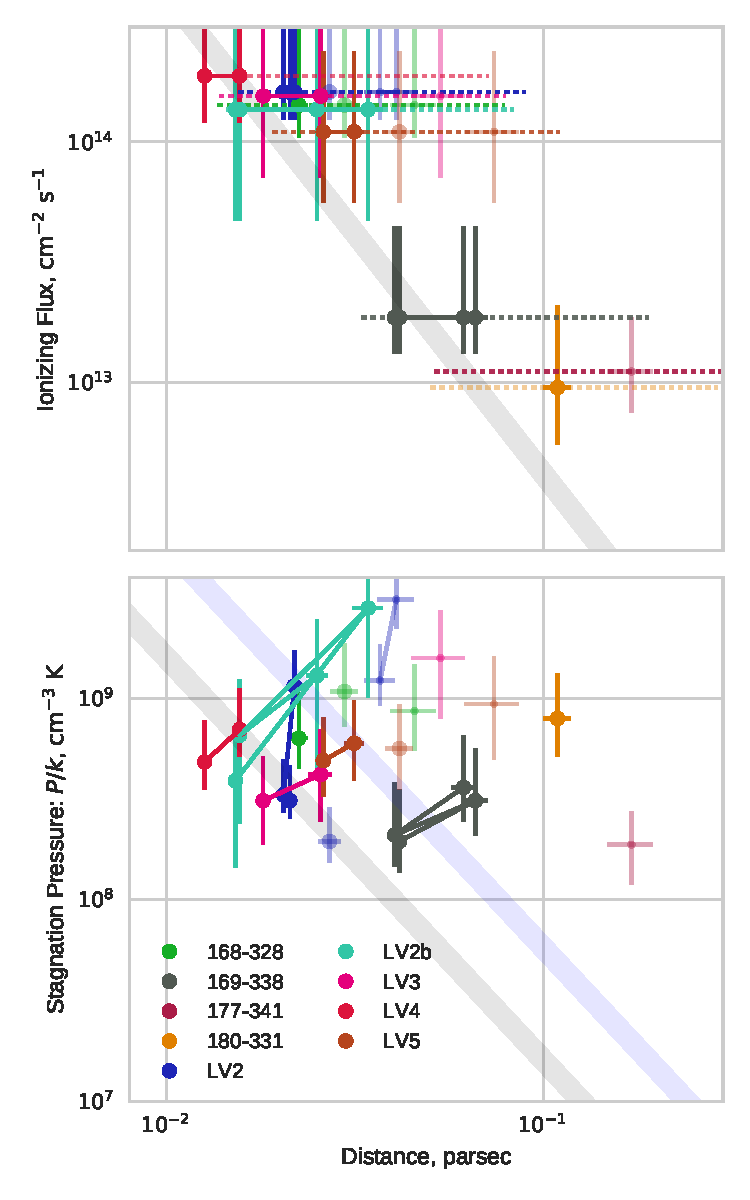
\includegraphics[width=0.5\linewidth]{./Figures/plot-wind-fits}& 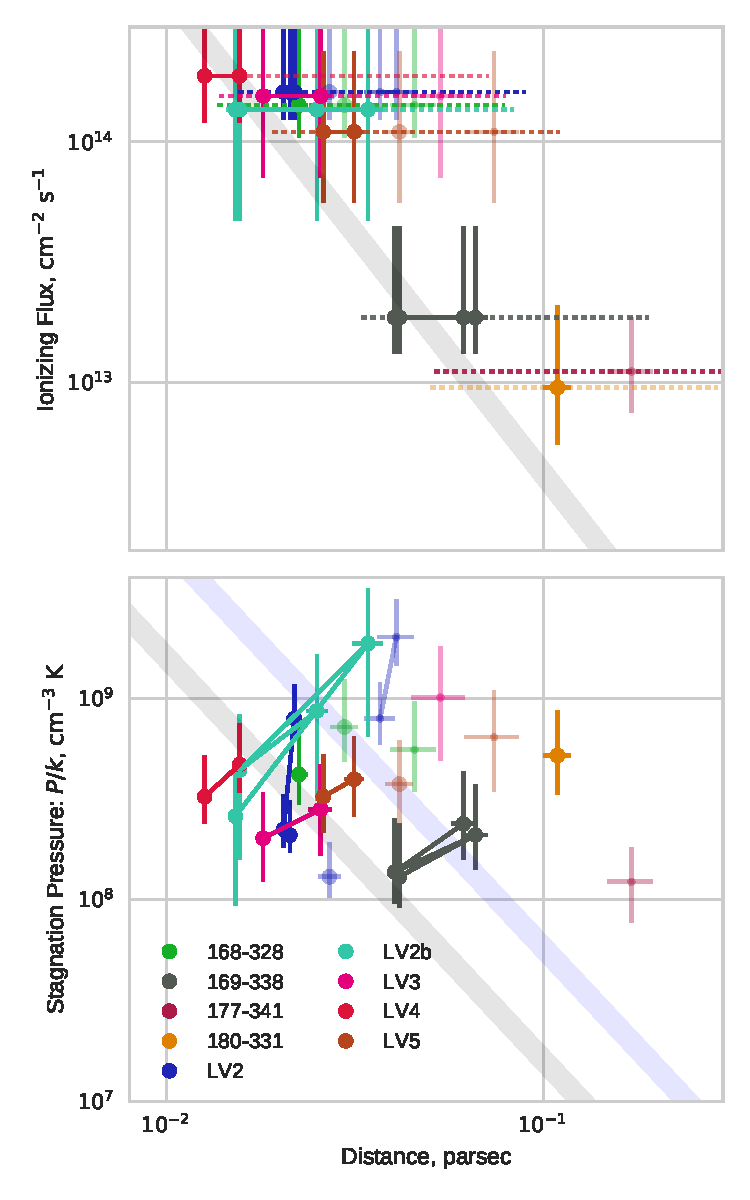
\includegraphics[width=0.5\linewidth]{./Figures/plot-wind-fits-2}  
  \end{tabular}
  \caption[Diagrama log-log de flujo y presión ram vs distancia para las sub-muestras de cada proplyd]{Diagrama log-log de flujo y presión ram vs distancia, para las sub-muestras de cada proplyd, mostradas con colores, mientras que el flujo y presión ram de la estrella se muestran con la línea gris. Las mediciones de la presión y el flujo utilizan las mediciones del radio del IF y densidad de la tabla \ref{tab:Prop-IF-par}, una tasa de fotones ionizantes de $\Nio_* = \SI{1e49}{s^{-1}}$, que corresponde a una estrella de tipo espectral entre O5 y O6 (ver tabla \ref{tab:ionizing-radiation}), un factor de absorción por polvo  $f_d$ de 0.5 y el IF de los proplyds es de tipo D-crítico. En el pánel izquierdo el número de Mach del flujo fotoionizado es $M=3$, y en el pánel derecho es $M=2$. En esta figura se muestra el modelo A: se utiliza la densidad y radio del frente de ionización de la tabla \ref{tab:Prop-IF-par}. En los diagramas de presión vs distancia, la línea azul representa la presión ram del viento de \thC{} del modelo \textit{frío} (azul) de \citet{Gagne:2005}, y en la lína gris se utilizan la tasa de pérdida de masa y la velocidad terminal reportados en \citet{GAH:2002}.}
  \label{fig:wind-fits}
\end{figure}

\begin{figure}
  \ContinuedFloat
  \captionsetup{list=off, format=cont}
  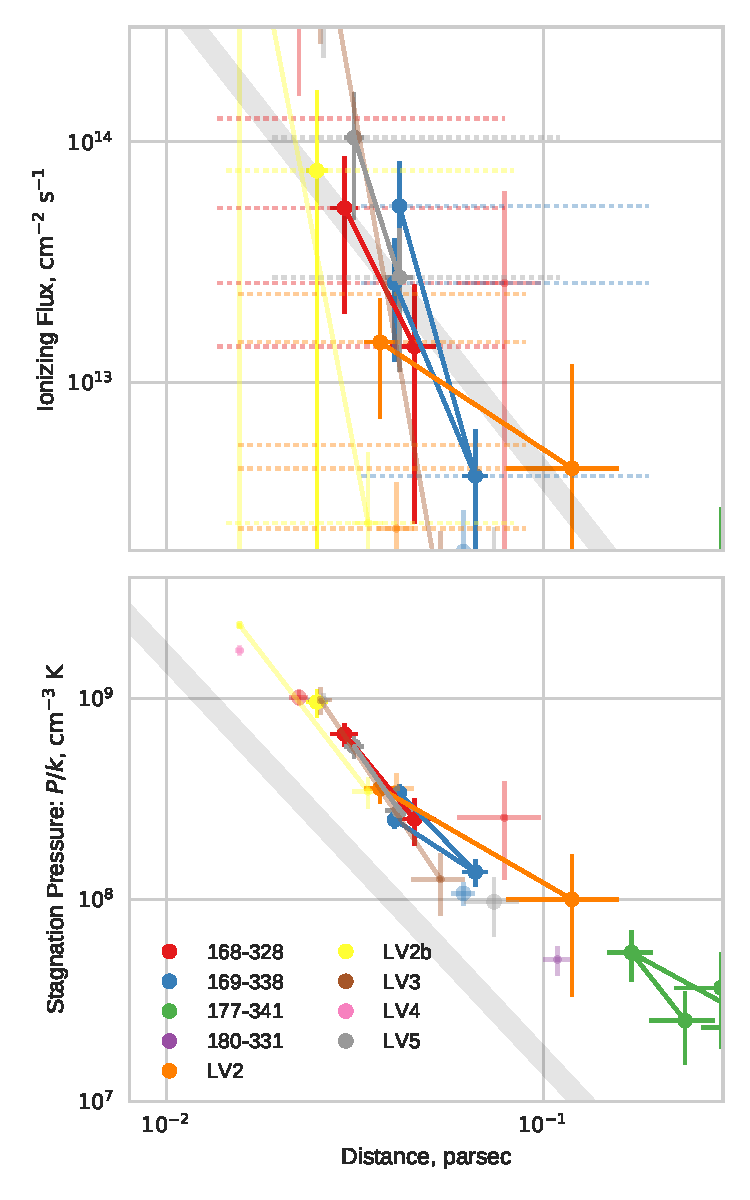
\includegraphics[width=0.5\linewidth]{./Figures/plot-wind-fits-beta}& 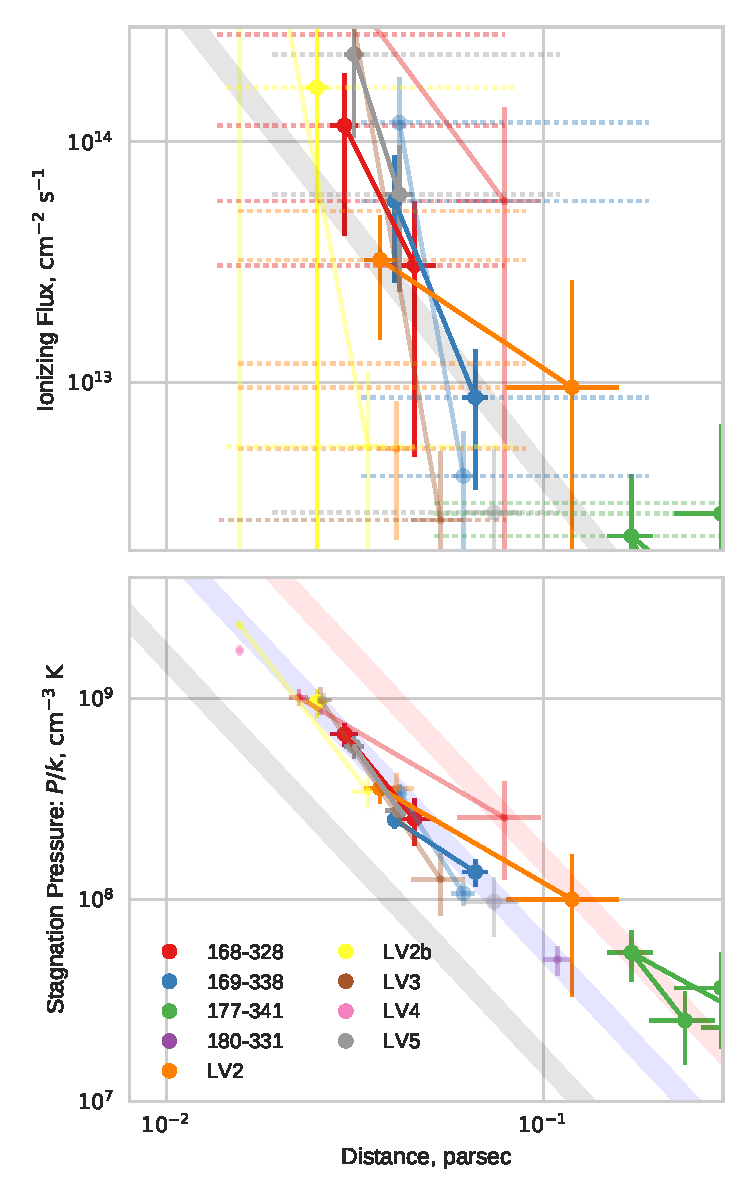
\includegraphics[width=0.5\linewidth]{./Figures/plot-wind-fits-beta-2}
  \caption{Modelo B.1: la densidad se obtiene de a partir de la tasa de momentos $\beta$ obtenida para cada submuestra con la ecuación \ref{eq:b-density}, y utilizando la tasa de pérdida de masa y la velocidad terminal del viento de \thC{} reportada en \citet{GAH:2002}.}
\end{figure}

\begin{figure}
  \ContinuedFloat
  \captionsetup{list=off, format=cont}
  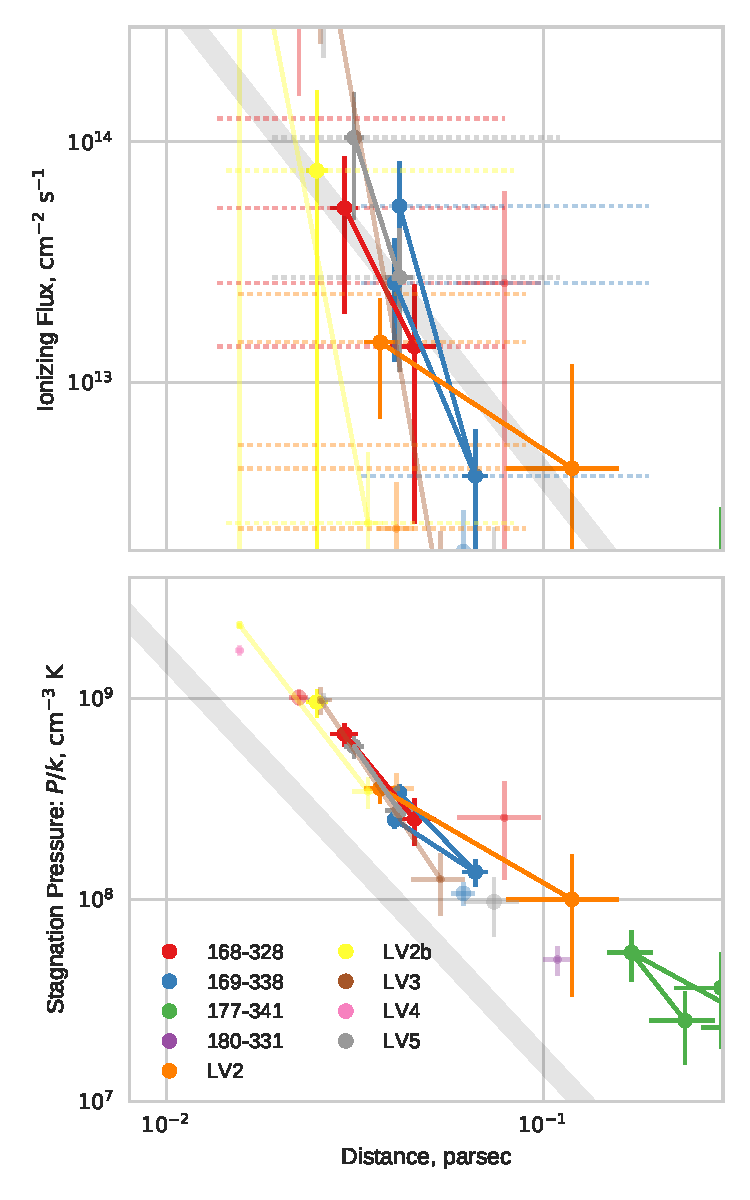
\includegraphics[width=0.5\linewidth]{./Figures/plot-wind-fits-beta}& 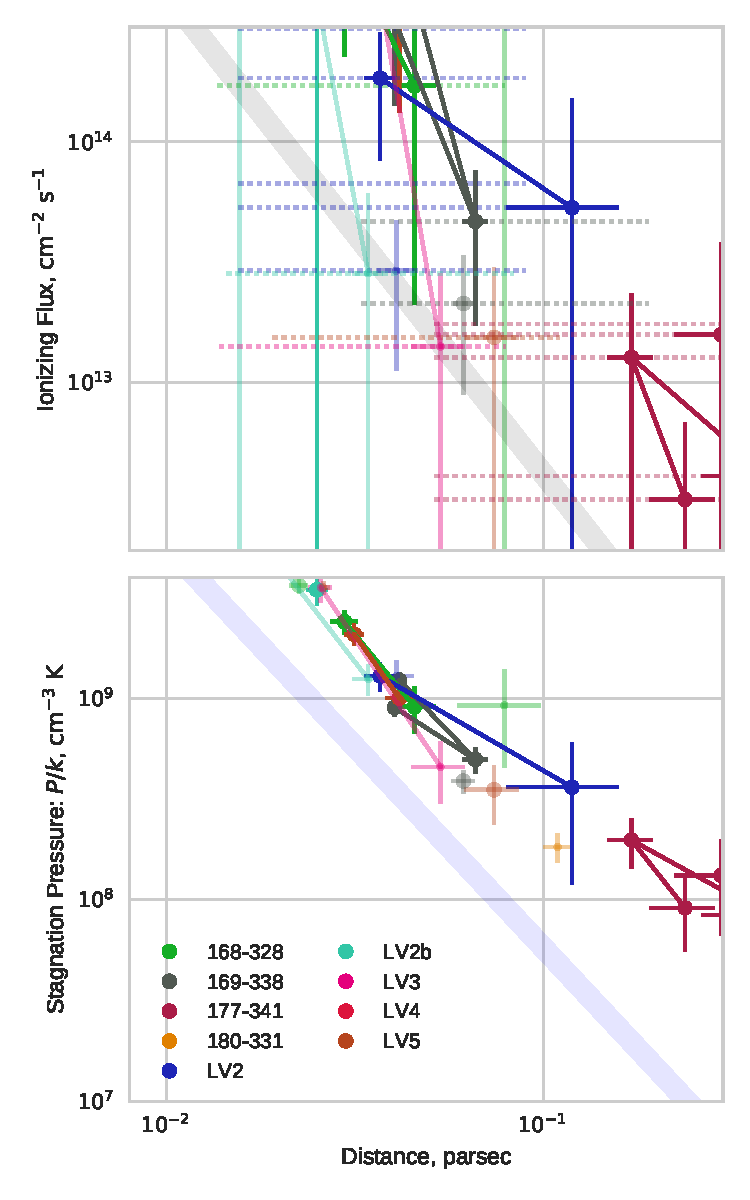
\includegraphics[width=0.5\linewidth]{./Figures/plot-wind-fits-beta-Gagne}
  \caption{Modelo B.2: la densidad se obtiene de a partir de la tasa de momentos $\beta$ obtenida para cada submuestra con la ecuación \ref{eq:b-density}, suponiendo que el número de Mach del viento interno es $M=3$ y utilizando la tasa de pérdida de masa y la velocidad terminal del viento de \thC{} del modelo \textit{frío} reportada en \citet{Gagne:2005}.}
\end{figure}

\begin{figure}
    \ContinuedFloat
    \captionsetup{list=off, format=cont}
    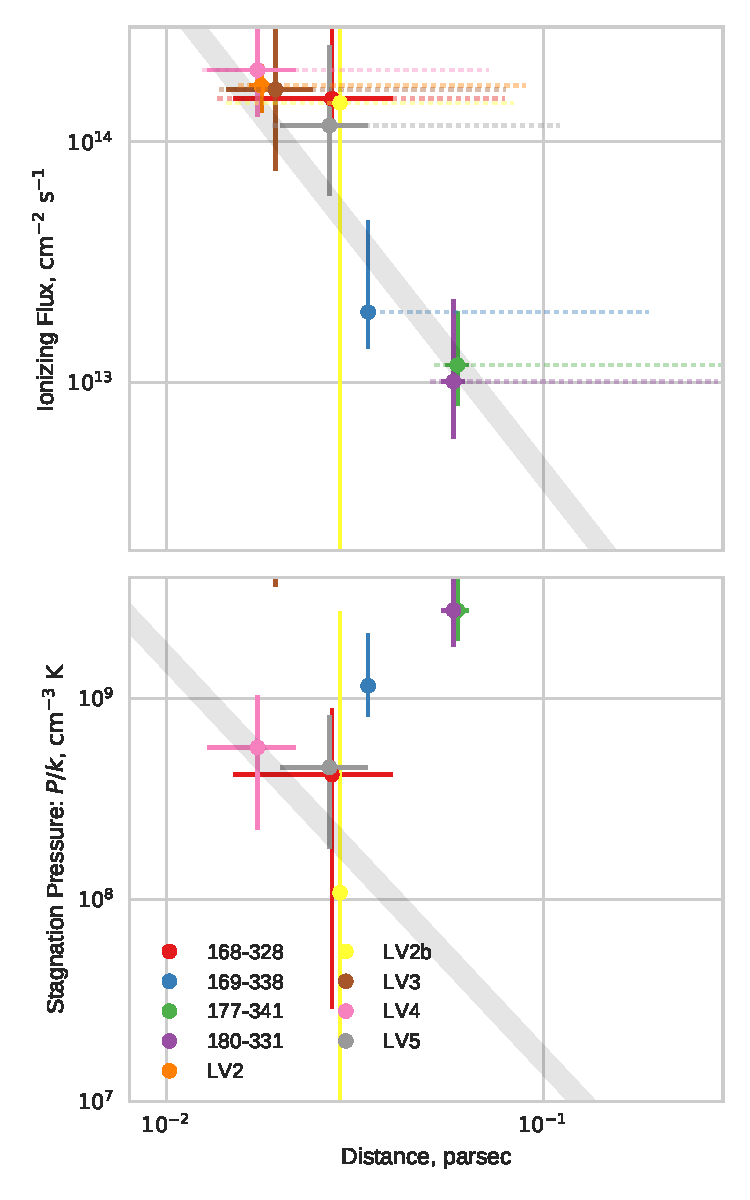
\includegraphics[width=0.5\linewidth]{./Figures/plot-wind-fits-HA98} & 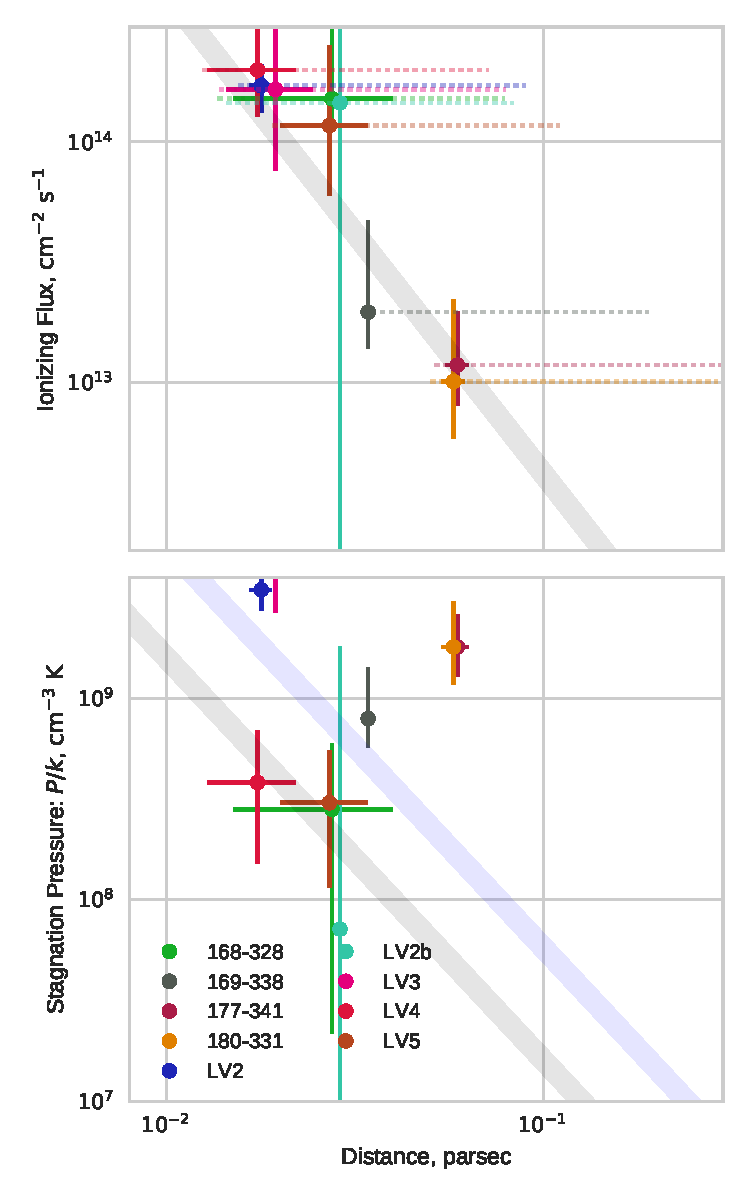
\includegraphics[width=0.5\linewidth]{./Figures/plot-wind-fits-HA98-2}
    \caption{Modelo HA, que utiliza las densidades de la tabla \ref{tab:Prop-IF-par} y además las inclinaciones reportadas en \citet{HA:1998}.}
\end{figure}


En la figura \ref{fig:wind-fits} mostramos diagramas log-log de flujo vs distancia y presión vs distancia de los proplyds (mostrados en colores) junto con el flujo y presión del viento de \thC{} (mostrados con la líneas gruesas semi-transparentes). En el diagrama de la presión, la línea azul representan dos modelos para el viento estelar de \thC{} utilizados en \citet{Gagne:2005}: el modelo \textit{frío} (azul), apropiado para una estrella O7, utiliza una tasa de pérdida de masa de $\dot{M}^0_{w1} = \SI{5.5e-7}{M_\odot.yr^{-1}}$ y una velocidad terminal del viento de $v_{w1} = \SI{2760}{km.s^{-1}}$, también existe el modelo \textit{caliente}, apropiado para una estrella tipo O5.5, utiliza una tasa de pérdida de masa de $\dot{M}^0_{w1} = \SI{1.4e-6}{M_\odot.yr^{-1}}$ y una velocidad del viento de $v_{w1} = \SI{2980}{km.s^{-1}}$ (en la línea gris la tasa de pérdida de masa es de $\dot{M}^0_{w1} = \SI{3.5e-7}{M_\odot.yr^{-1}}$ y la velocidad terminal del viento es de $v_{w1} = \SI{1400}{km.s^{-1}}$, \citet{GAH:2002}). Sin embargo, los diferentes métodos para determinar los parámetros del viento de \thC{} llevan a calcular el cociente $\dot{M}_{w1}/v_{w1}$ en vez de dichos parámetros en particular. Entonces se asume un valor plausible para la velocidad terminal $v_{w1}$ del viento y en consecuencia se estima la tasa de pérdida de masa \citep{Garcia-Arredondo:2001}. Midiendo el ancho equivalente de la línea de \Ion{H}{\alpha}, se encuentra un cociente de $\dot{M}_{-7}/v_{3} = 3.85$, donde $\dot{M}_{-7}$ es la tasa de pérdida de masa medida en unidades de \SI{e-7}{M_\odot.yr^{-1}}, y $v_3$ es la velocidad terminal del viento en unidades de \SI{e3}{km.s^{-1}} \citep{Garcia-Arredondo:2001}. Sin embargo, existe una variabilidad en el viento de \thC{} y probablemente el valor de  $\dot{M}_{-7}/v_{3}$ encontrado mediante el ancho equivalente de \Ion{H}{\alpha} sea un límite superior, y que el valor promedio de este cociente sea aproximadamente la mitad, es decir, $\dot{M}_{-7}/v_{3} \simeq 1.9$. En \citet{Garcia-Arredondo:2001} se aplica el criterio adicional de que $\dot{M}_{w1}v_{w1} = 4.2$ para que se cumpla la condición de equilibrio de presión ram de LV2 a una inclinación de $i=50^\circ$ (equivalente a $40^\circ$ en este trabajo, siendo que el ángulo de inclinación utilizado en \citet{Garcia-Arredondo:2001} es el ángulo complementario de la inclinación utilizada en este trabajo). De esta forma la tasa de pérdida de masa $\dot{M}^0_{w1} = \SI{3.5e-7}{M_\odot.yr^{-1}}$ y la velocidad terminal $v_{w1} = \SI{1400}{km.s^{-1}}$ cumplen estos criterios. Por otro lado, en el modelo \textit{caliente} de \citet{Gagne:2005} se encuentra que $\dot{M}_{-7}/v_{3} \simeq 4.7$, demasiado alto respecto a lo que predice el ancho equivalente de la línea de \Ion{H}{\alpha}, por lo tanto, es poco realista utilizarlo para modelar el viento de \thC{}. Sin embargo, el modelo \textit{frío} predice que $\dot{M}_{-7}/v_{3} \simeq 2$, ligeramente por encima del $1.9$ que predice el ancho equivalente de la línea de \Ion{H}{\alpha}, por lo que si relajamos el criterio de que $\dot{M}_{w1}v_{w1} = 4.2$ entonces este modelo no es totalmente descartable.

En todos los casos utilizamos el radio del frente de ionización reportado en \citet{Garcia-Arredondo:2001}, tabla 1, pero escalados a la distancia a ONC utilizada en este trabajo ($414 \pm \SI{6.8}{pc}$, \citet{Menten:2007}), y mostrados en la columna 3 de la tabla \ref{tab:Prop-IF-par}, para la densidad utilizamos dos modelos diferentes:

\begin{enumerate}[A.]
\item Utilizando los perfiles de brillo y la densidad máxima del frente de ionización obtenidos en \citet{Garcia-Arredondo:2001}, pero escalando por la distancia a \thC{} (columna 4 de la tabla \ref{tab:Prop-IF-par})
\item A partir de nuestras propias mediciones de la tasa de momentos $\beta$, y utilizando las ecuaciones (\ref{eq:beta-def}, \ref{eq:inner-dot-M}) la densidad se calcula como sigue:

  \begin{align}
    n_{ps} = \frac{\beta\left(\dot{M}^0_{w1}v_{w1}\right)\left(k + 1\right)}{2\pi R^2_0 \bar{m}\left(M c_{\mathrm{II}}\right)^2} \label{eq:b-density}
  \end{align}
\item Como referencia mostramos el modelo GAH, donde utilizamos las densidades de la columna 4 de la tabla \ref{tab:Prop-IF-par} y las inclinaciones reportadas en \citet{HA:1998}, tabla 2, excepto por LV2, donde la inclinación es corregida a $i=40^\circ \pm 10^\circ$ \citep{Henney:2002, Garcia-Arredondo:2001}.
\end{enumerate}


Para todos los modelos, suponemos que el número de Mach del flujo fotoevaporado en la posición del choque es de $M=[2, 3]$, que es un intervalo plausible para la velocidad del flujo fotoevaporado. Algunas observaciones cualitativas son las siguientes: la variación con el número de Mach en la presión en los Modelos A y HA es pequeña (la diferencia entre los diagramas con $M=3$ y $M=2$ es de $\log\left(\frac{P_{\mathrm{in}}(M=2)}{P_{\mathrm{in}}(M=3)}\right)\simeq -0.35$) mientras que en el modelo B no existe variación en la presión con velocidad pero sí en el flujo, a través de las ecuaciones (\ref{eq:F-ph}, \ref{eq:density-scale} y \ref{eq:b-density}). Debido a la dependencia de la densidad del viento interior con los parámetros del viento exterior en el modelo B, éste está subdividido en modelo B.1, donde se usan los parámetros del viento exterior de \citet{GAH:2002}, y modelo B.2, donde se utilizan los parámetros del modelo \textit{frío} de \citet{Gagne:2005} (ver continuación de la figura \ref{fig:wind-fits}). Otra observación importante es que en los modelos A y GAH no parece existir una correlación entre las presiones ram de los proplyds con su distancia a \thC{}, aunque algunos proplyds se encuentran en equilibrio de presión con el viento de \thC{}. Por otro lado, en el modelo B la presión ram del viento interior es proporcional a $D^{-2}$, pero está por encima de la presión ram del viento de \thC{}. %También se observa que los proplyds más lejanos, 177-341 y 180-331 están por encima de equilibrio de presión en los tres modelos para la densidad. Esto puede deberse a que a estas distancias la presión del viento estelar deja de ser dominante y otros factores empiezan a ser importantes (ver por ejemplo \citet{GAH:2002}). Esto también puede atribuirse a que el viento de \thC{} no sea isotrópico.

Los resultados de este capítulo serán enviados a una revista próximamente.
